\documentclass[preprint,12pt,authoryear]{elsarticle}
%\documentclass[review]{elsarticle}

\usepackage[colorlinks]{hyperref}
\usepackage{lineno}

\modulolinenumbers[5]

\journal{Ocean Engineering}

\usepackage{amssymb}
\usepackage{amsmath}


\usepackage{subfigure}

\usepackage{epstopdf}
\usepackage{epsfig}
\usepackage{setspace}

\usepackage{ulem}

\newcommand{\be}{\begin{equation}}
\newcommand{\ee}{\end{equation}}
\newcommand{\beq}{\begin{eqnarray}}
\newcommand{\eeq}{\end{eqnarray}}
\newcommand{\ba}{\begin{eqnarray}}
\newcommand{\ea}{\end{eqnarray}}


%%%add
%\documentclass{article}
%\usepackage{natbib}
%\usepackage{cite}
\usepackage{soul}
\doublespacing
\usepackage{color}

%\renewcommand{\tablename}{Table}
\newcommand{\tabincell}[2]{\begin{tabular}{@{}#1@{}}#2\end{tabular}}

\newcommand{\ua}{{\bf u}_\alpha}
\newcommand{\utwo}{\overline{\bf u}_2}



\begin{document}


\begin{frontmatter}

\title{Modeling the optical signature induced by wave breaking using the Boussinesq-type wave model FUNWAVE-TVD
}


\author[first]{xxx}

\address[first]{xxx}

\begin{abstract}


\end{abstract}


\begin{keyword}

\end{keyword}

\end{frontmatter}

\linenumbers

\section{Introduction}


\begin{figure}
\centering
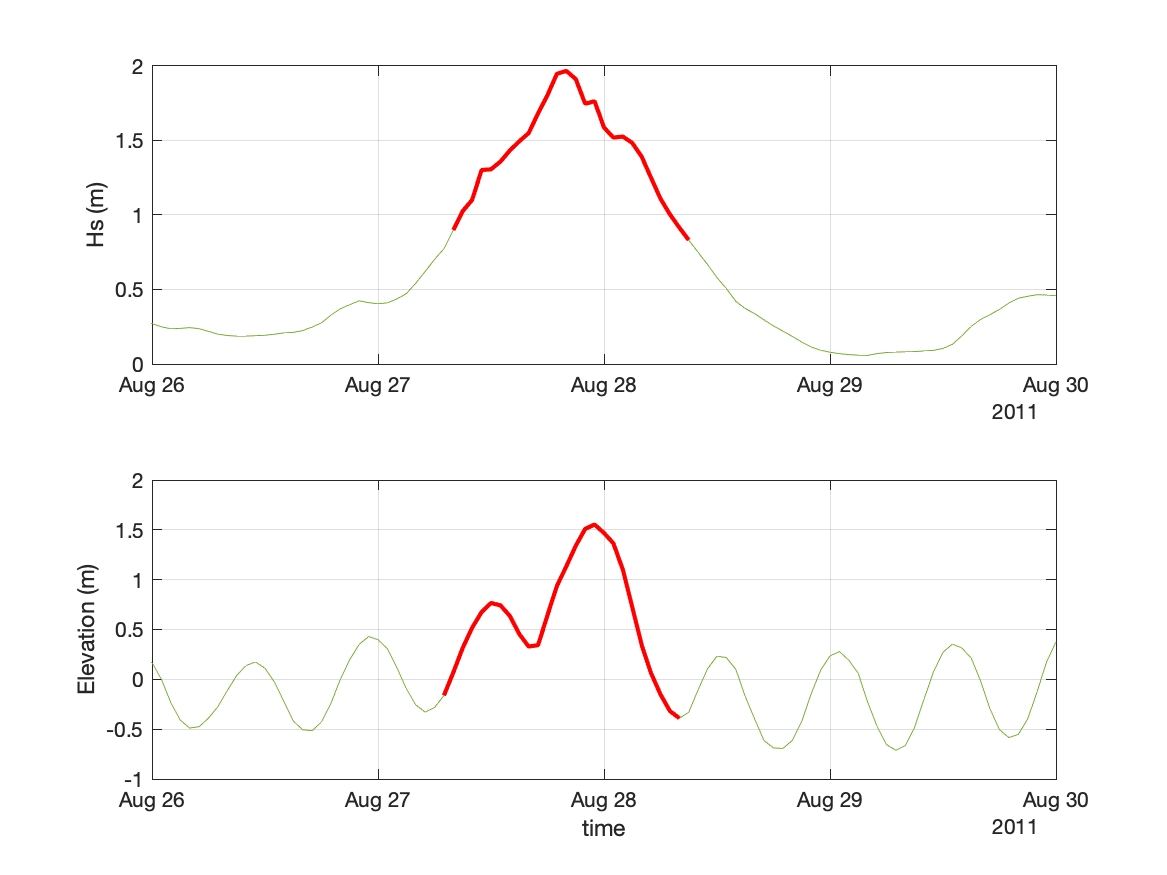
\includegraphics[width=\textwidth]{./figures/nearcom_wave_flow.jpg}
\caption{xxx }
\label{boundary}
\centering
\end{figure}

\begin{figure}
\centering
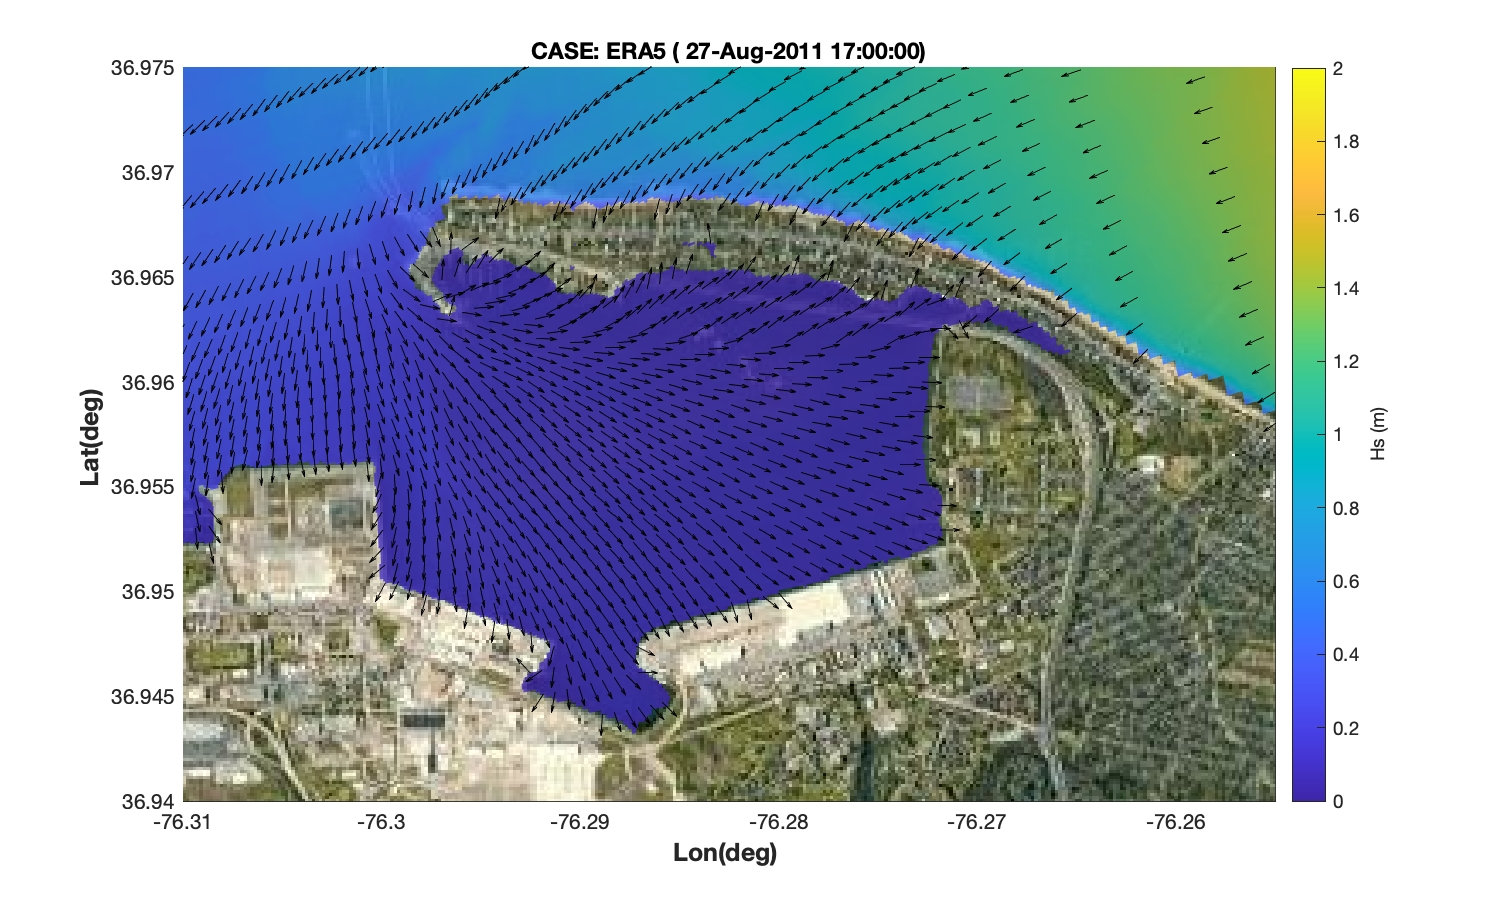
\includegraphics[width=\textwidth]{./figures/nearcom_hs_ERA5_55.jpg}
\caption{xxx }
\label{boundary}
\centering
\end{figure}

\begin{figure}
\centering
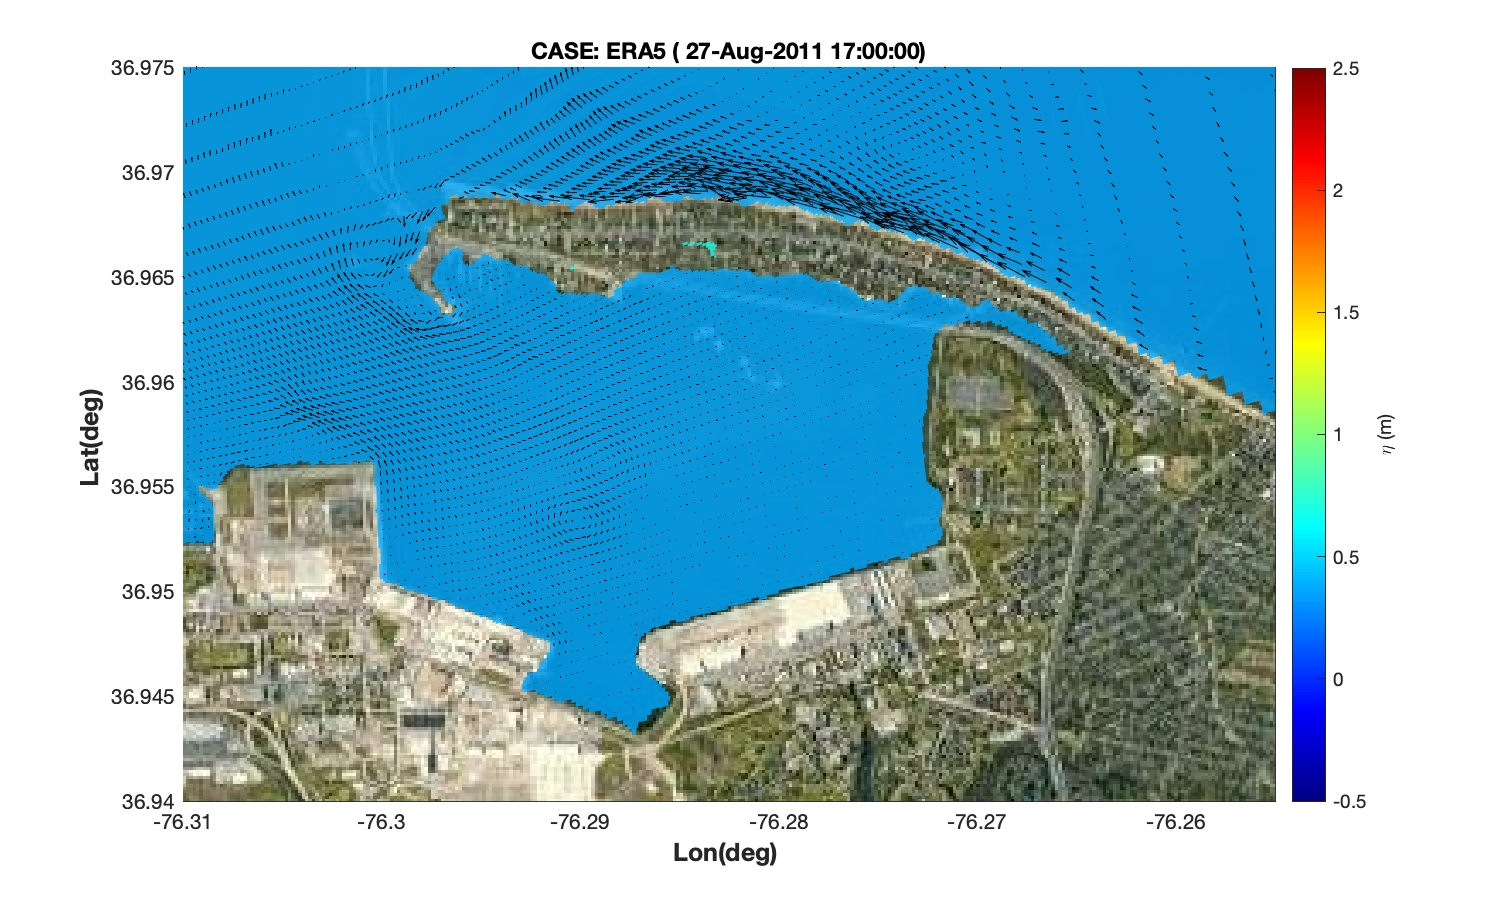
\includegraphics[width=\textwidth]{./figures/nearcom_ele_ERA5_55.jpg}
\caption{xxx }
\label{boundary}
\centering
\end{figure}

\begin{figure}
\centering
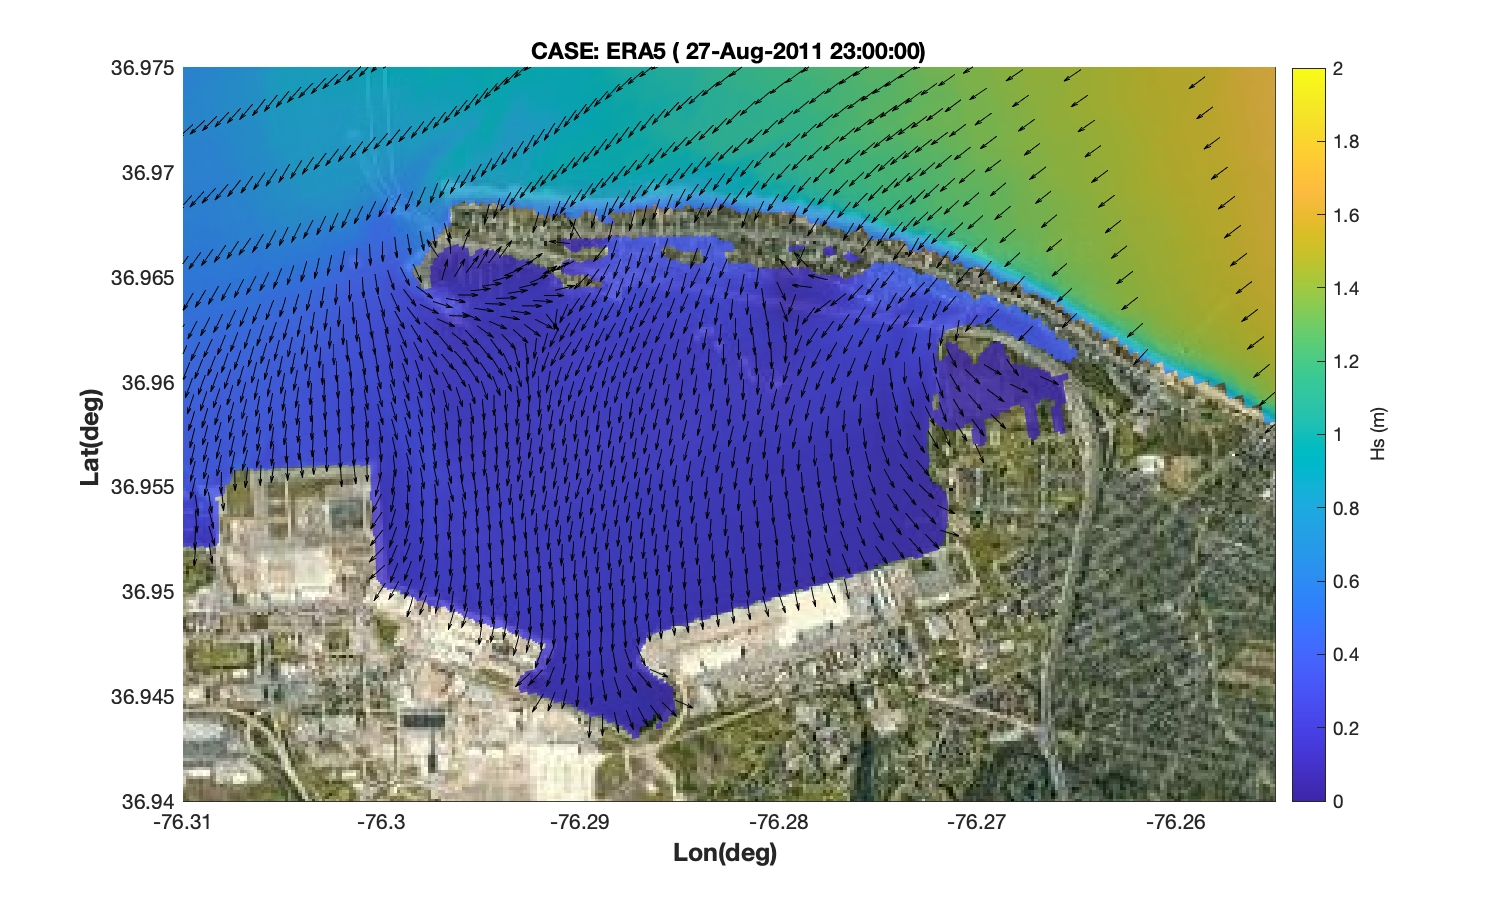
\includegraphics[width=\textwidth]{./figures/nearcom_hs_ERA5_91.jpg}
\caption{xxx }
\label{boundary}
\centering
\end{figure}

\begin{figure}
\centering
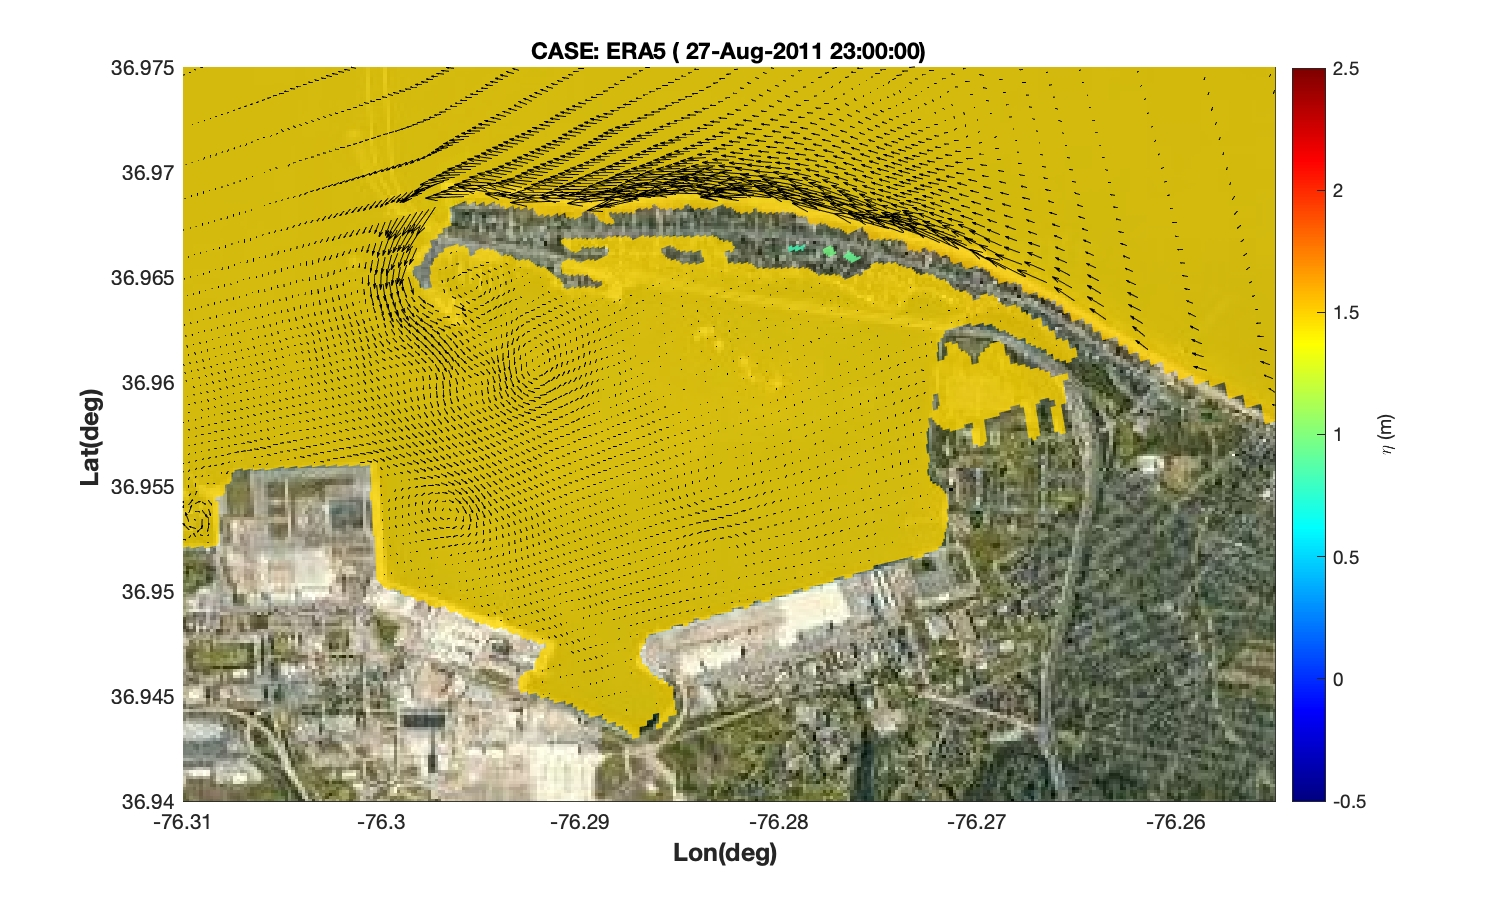
\includegraphics[width=\textwidth]{./figures/nearcom_ele_ERA5_91.jpg}
\caption{xxx }
\label{boundary}
\centering
\end{figure}

\begin{figure}
\centering
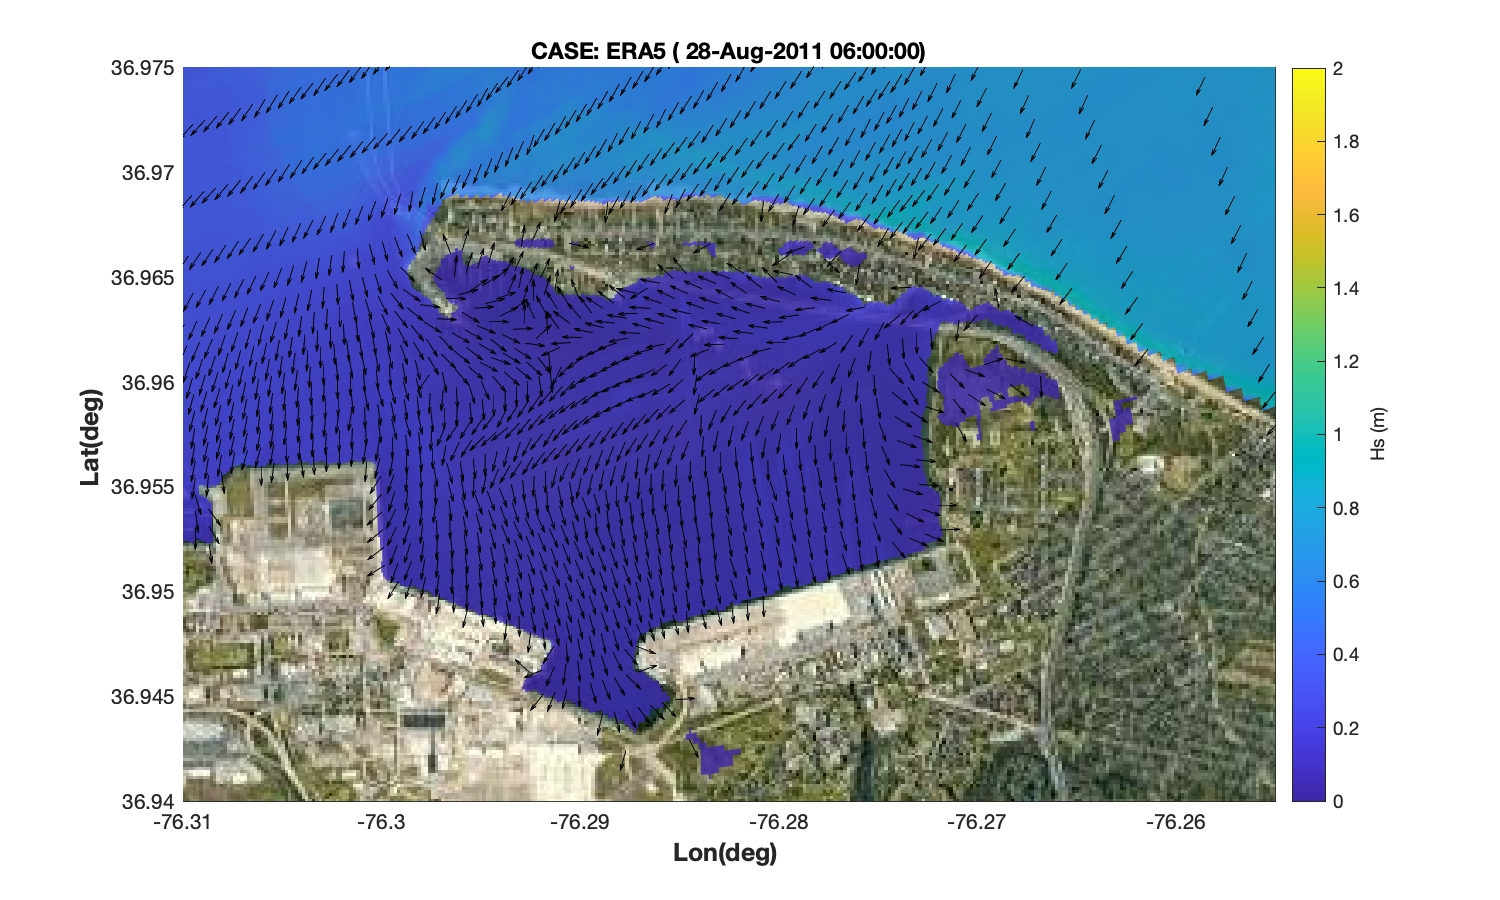
\includegraphics[width=\textwidth]{./figures/nearcom_hs_ERA5_133.jpg}
\caption{xxx }
\label{boundary}
\centering
\end{figure}

\begin{figure}
\centering
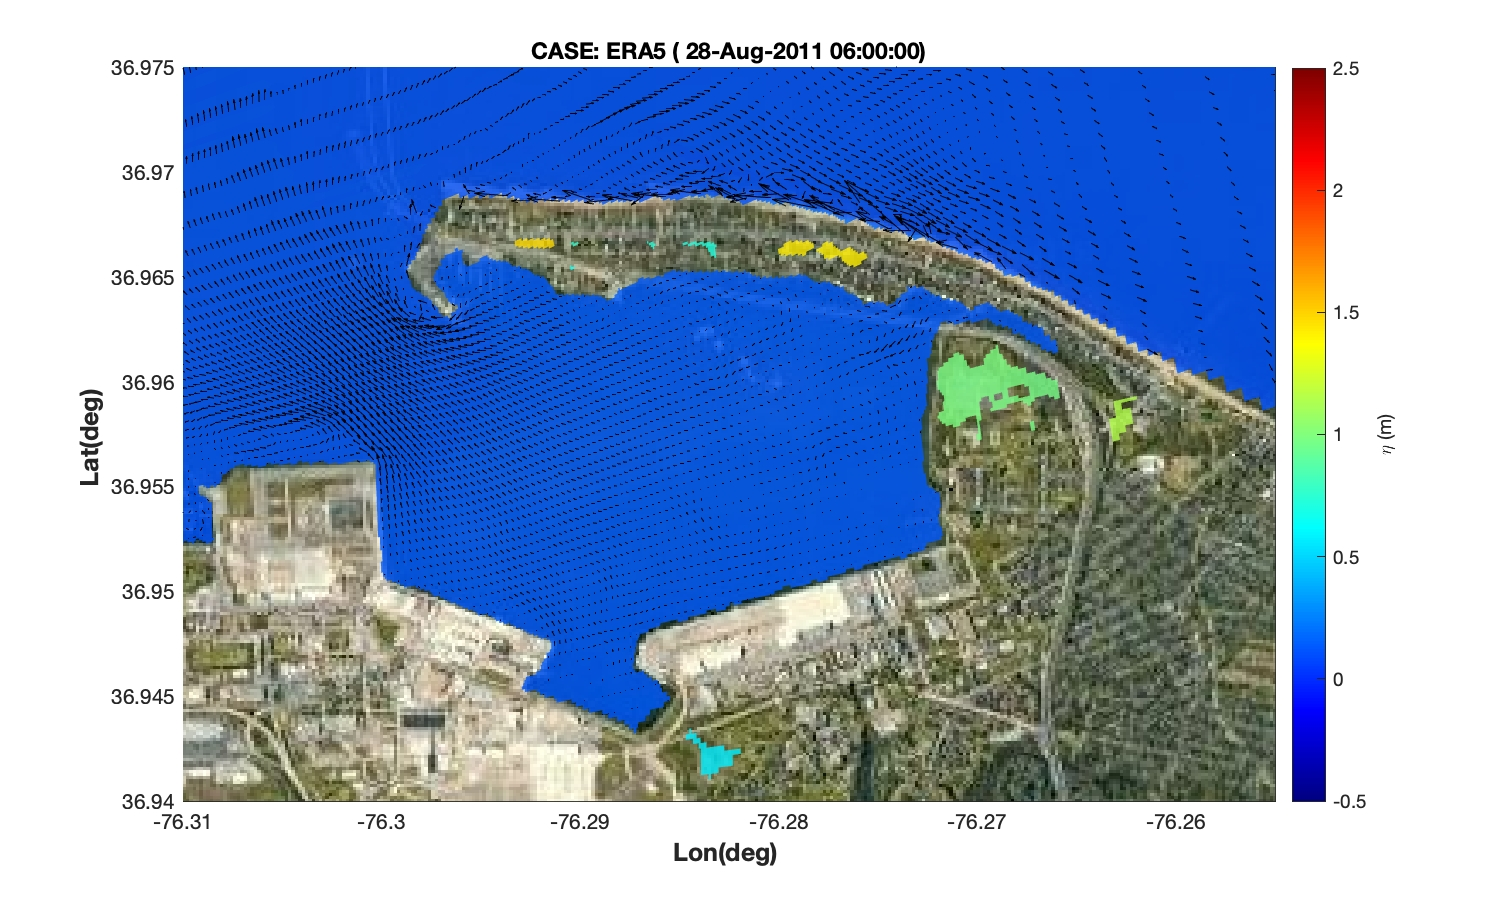
\includegraphics[width=\textwidth]{./figures/nearcom_ele_ERA5_133.jpg}
\caption{xxx }
\label{boundary}
\centering
\end{figure}

% wave versus no wave

\begin{figure}
\centering
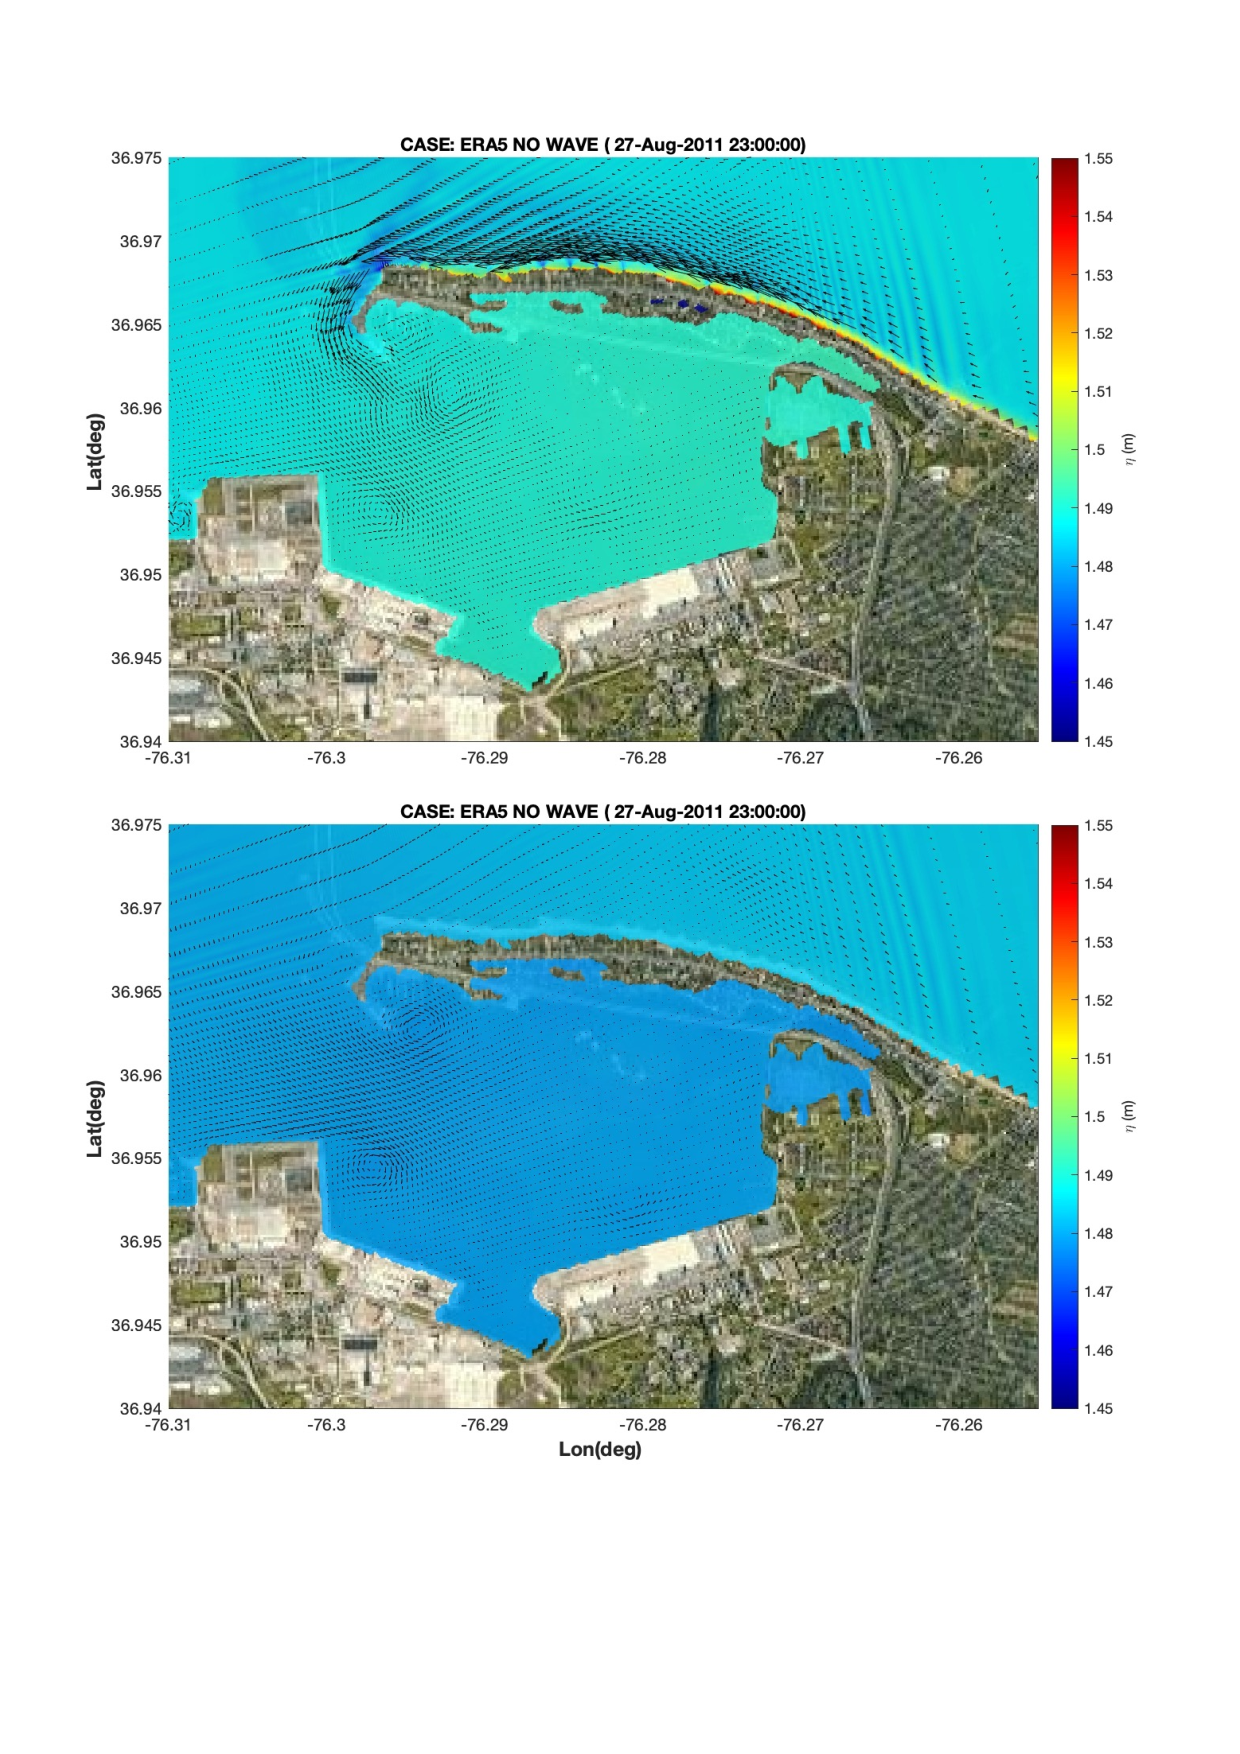
\includegraphics[width=\textwidth]{./figures/nearcom_wo_wave.pdf}
\caption{xxx }
\label{boundary}
\centering
\end{figure}


\begin{figure}
\centering
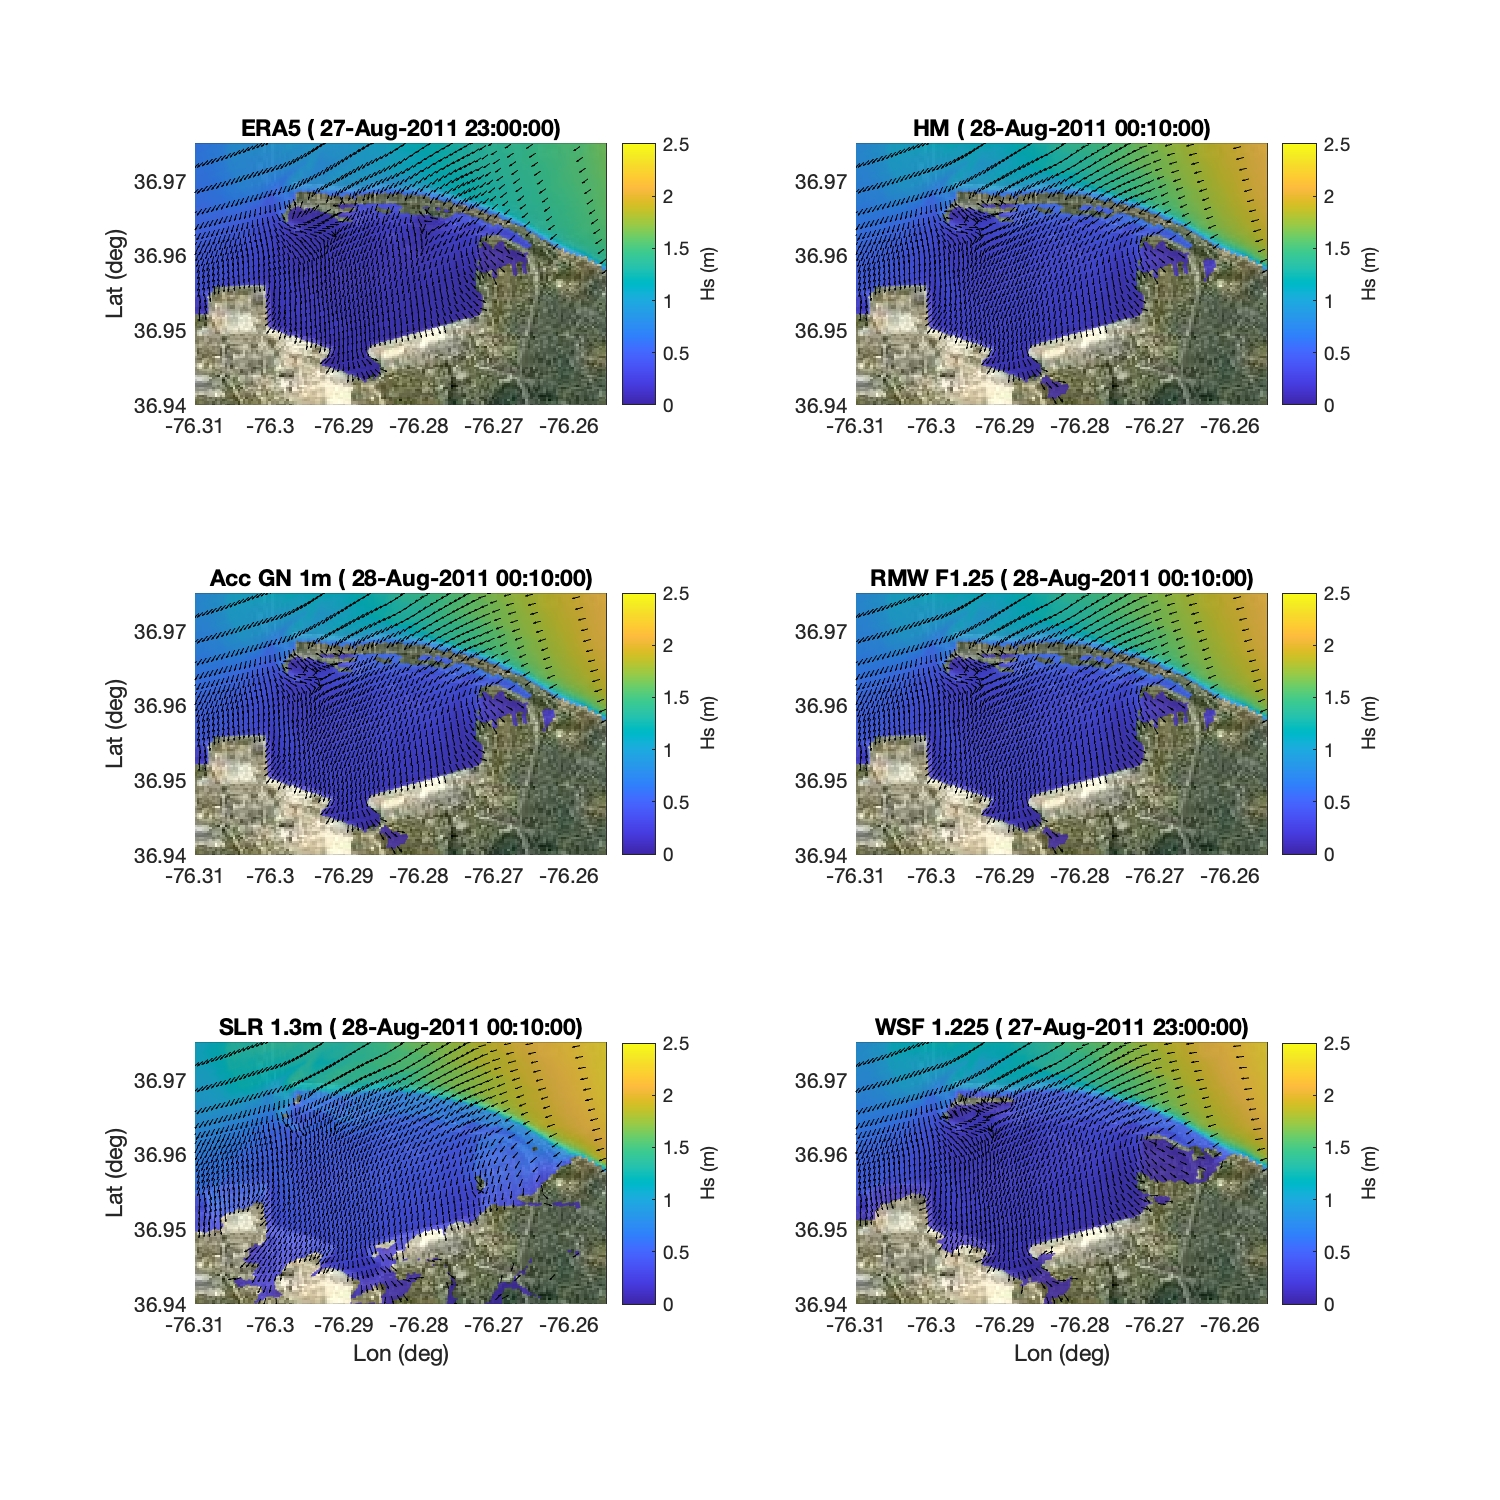
\includegraphics[width=\textwidth]{./figures/nearcom_hs.jpg}
\caption{xxx }
\label{boundary}
\centering
\end{figure}

\begin{figure}
\centering
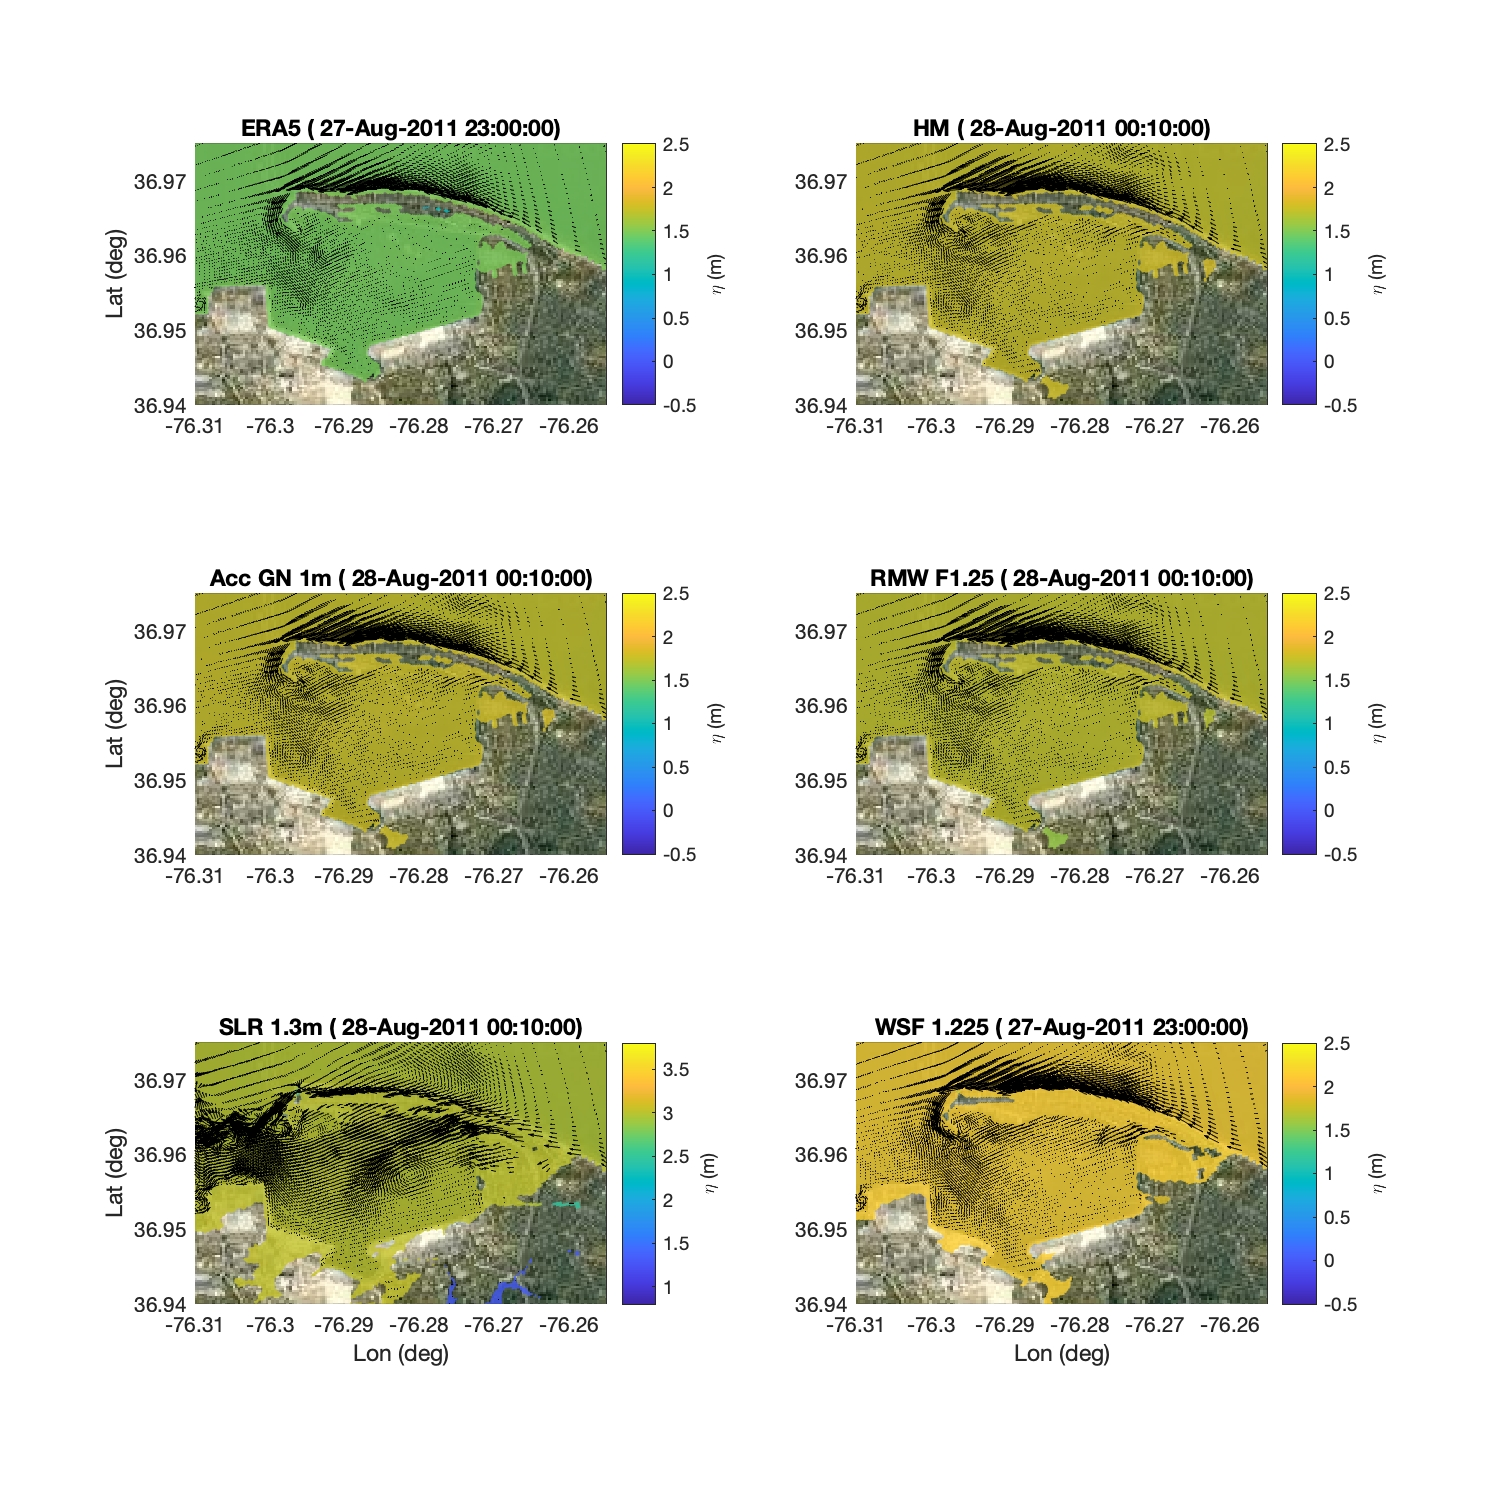
\includegraphics[width=\textwidth]{./figures/nearcom_eta_uv.jpg}
\caption{xxx }
\label{boundary}
\centering
\end{figure}

\begin{figure}
\centering
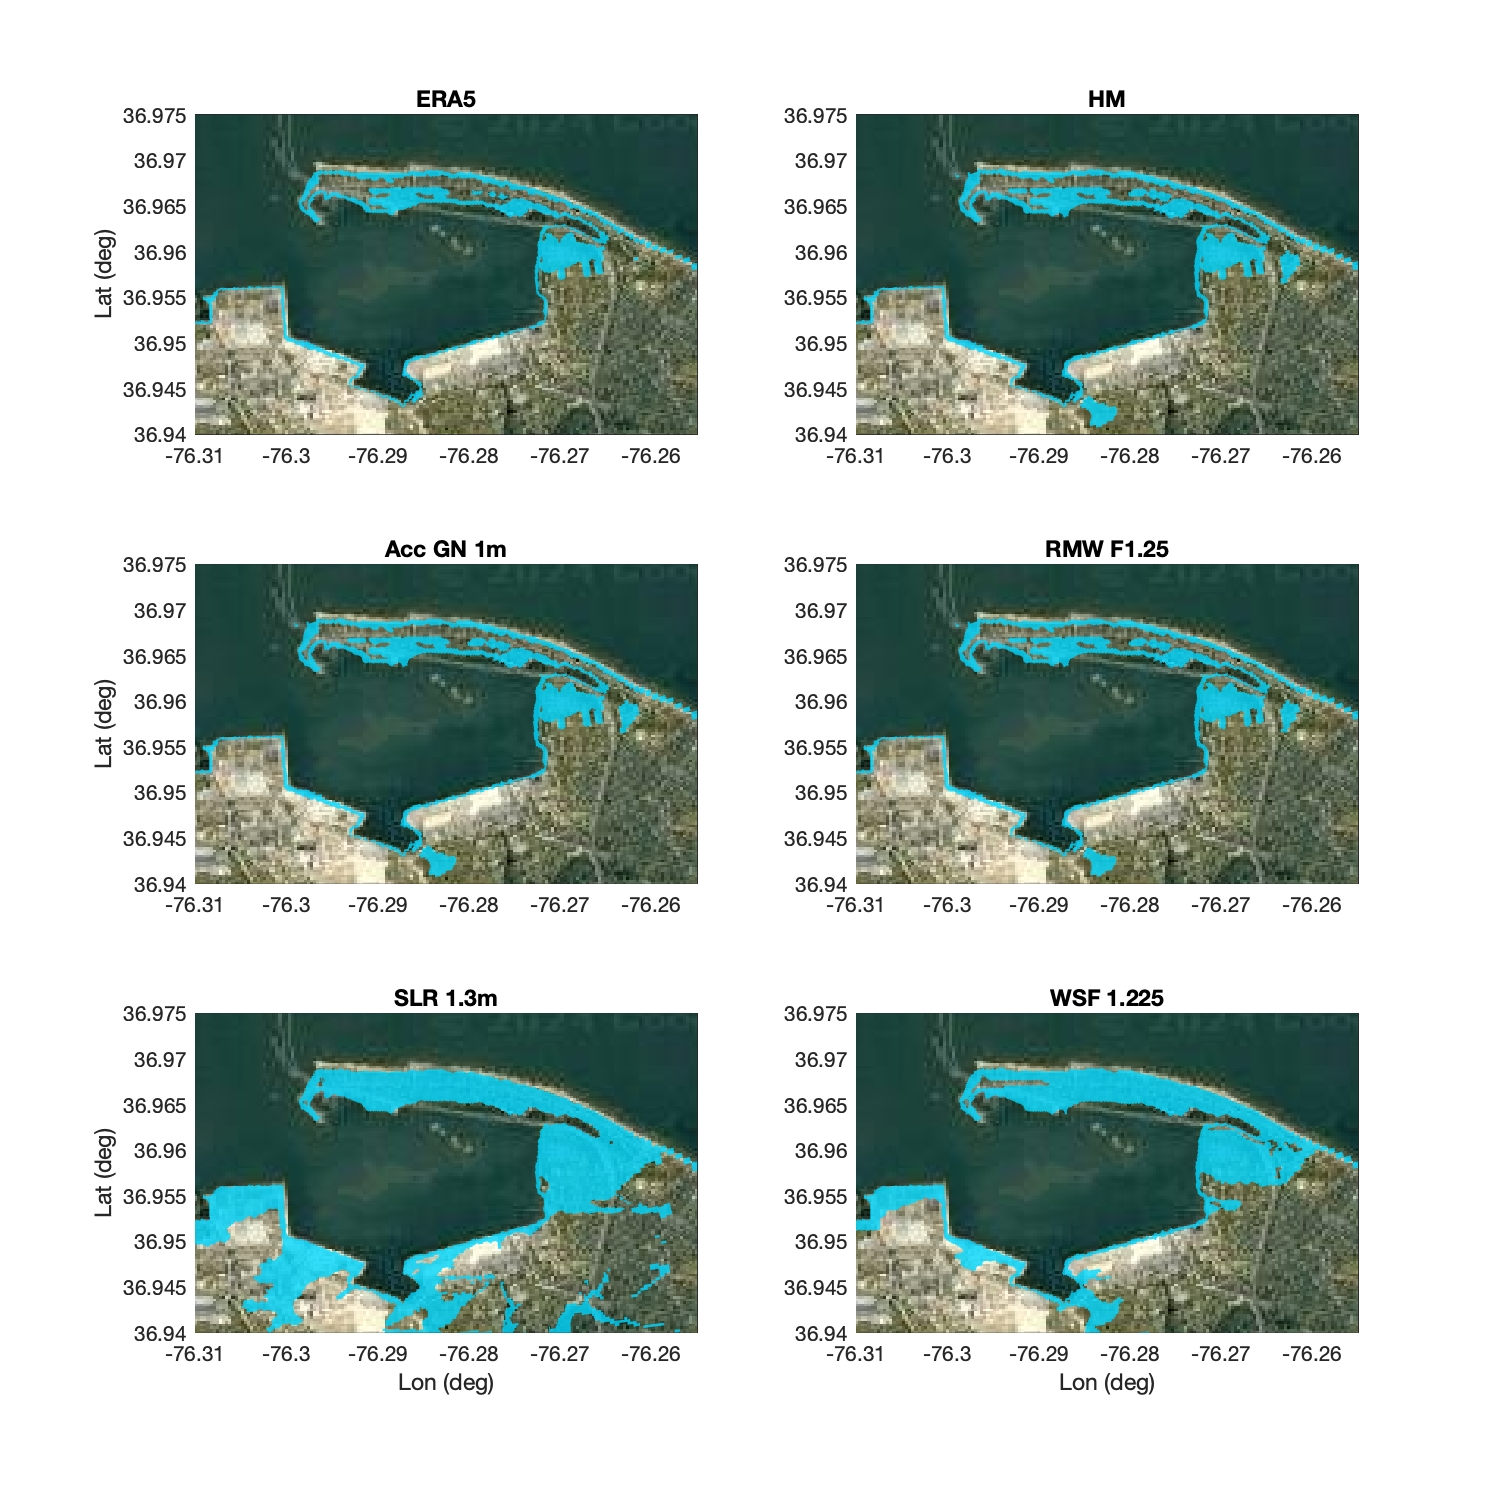
\includegraphics[width=\textwidth]{./figures/nearcom_flood.jpg}
\caption{xxx }
\label{boundary}
\centering
\end{figure}

\begin{figure}
\centering
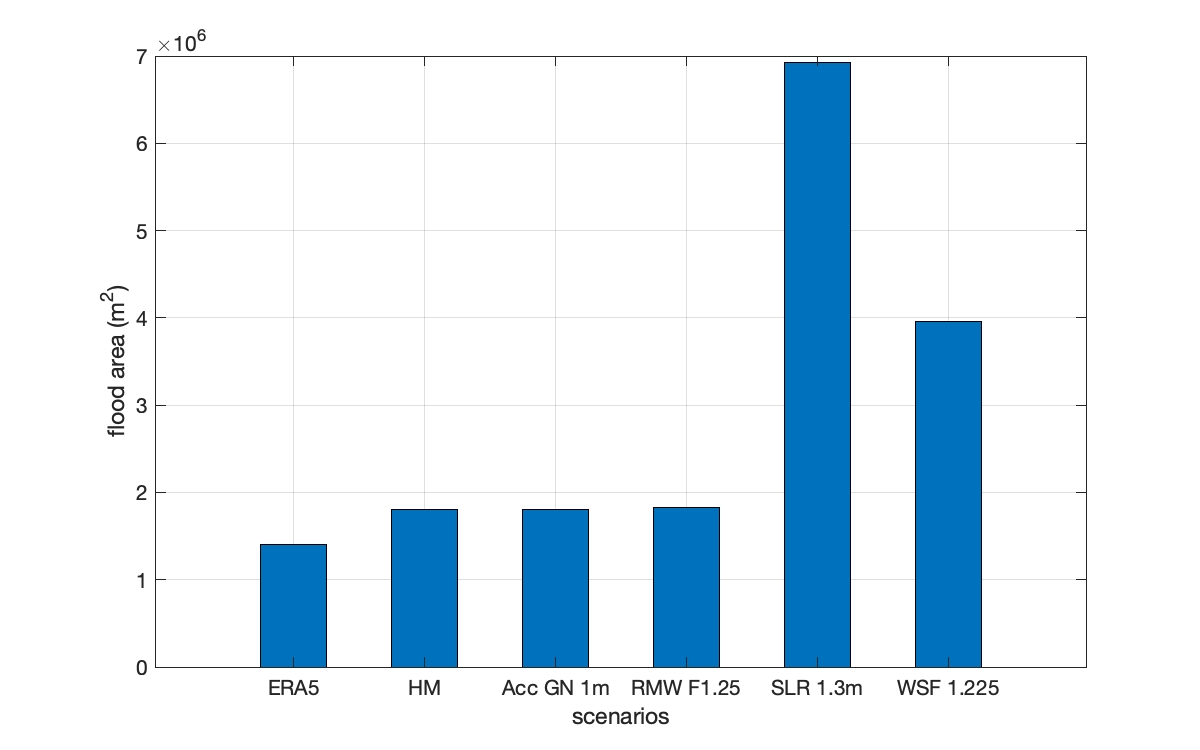
\includegraphics[width=\textwidth]{./figures/nearcom_bars.jpg}
\caption{xxx }
\label{boundary}
\centering
\end{figure}

% funwave

\begin{figure}
\centering
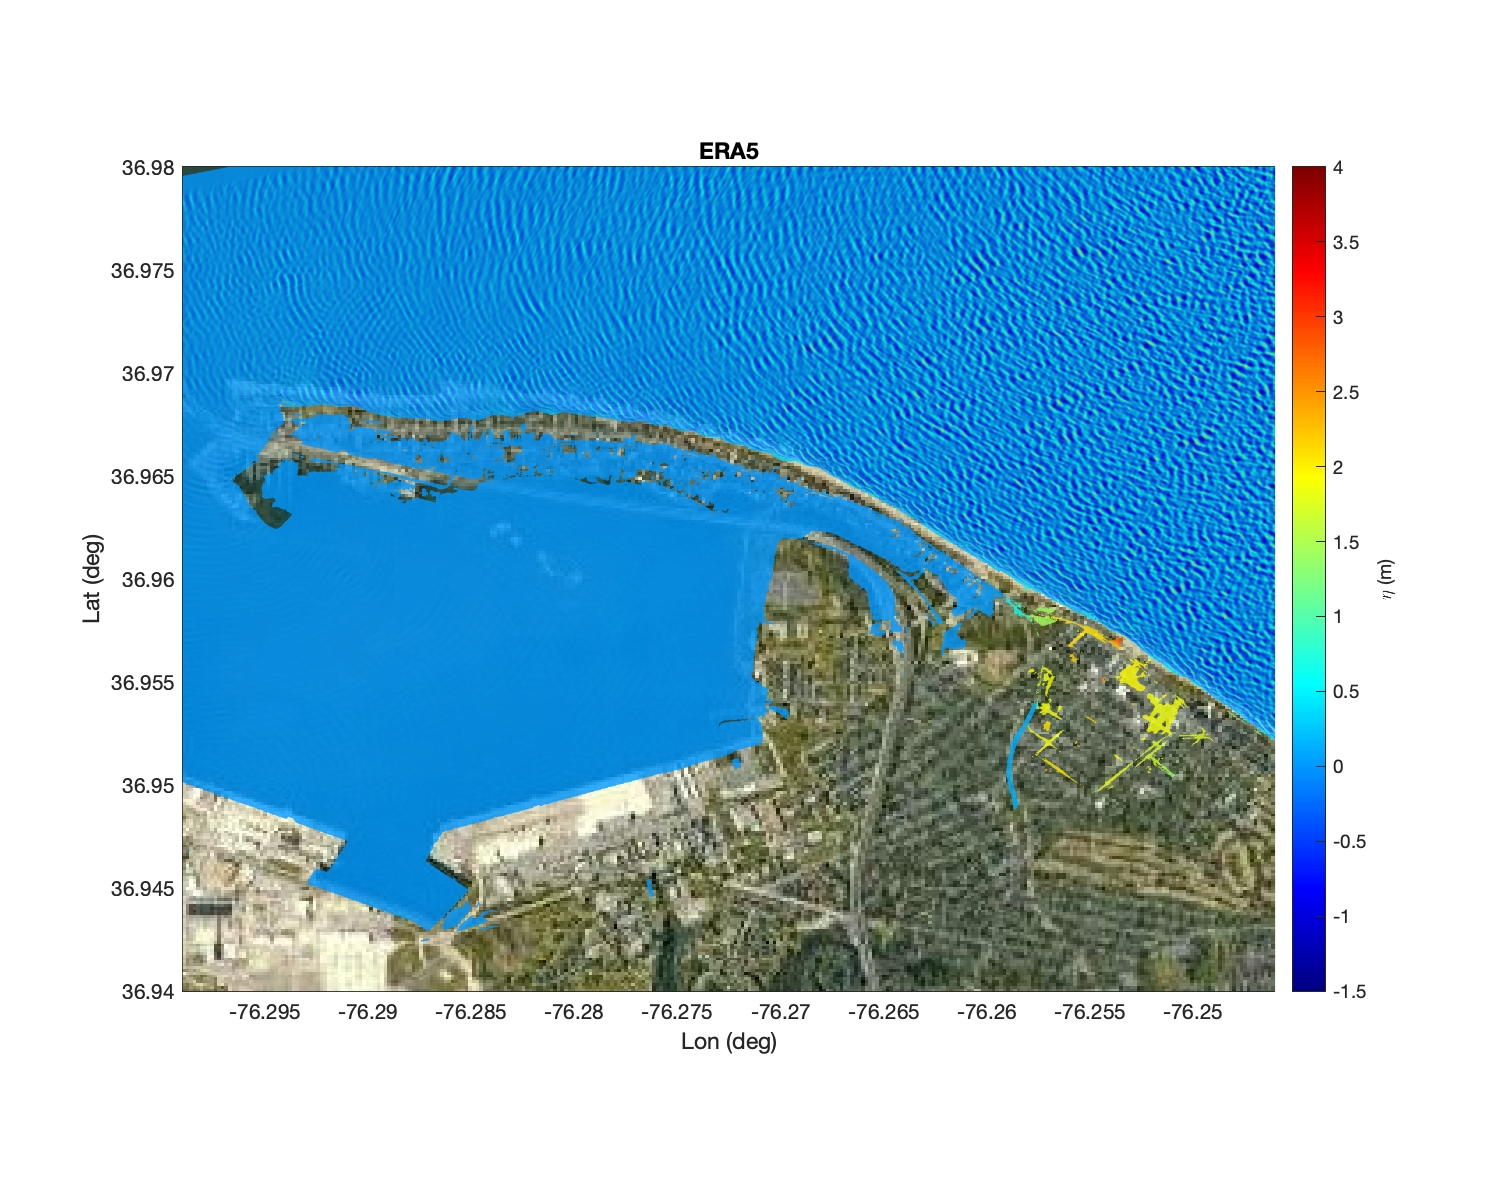
\includegraphics[width=\textwidth]{./figures/funwave_ERA5_eta.jpg}
\caption{xxx }
\label{boundary}
\centering
\end{figure}

\begin{figure}
\centering
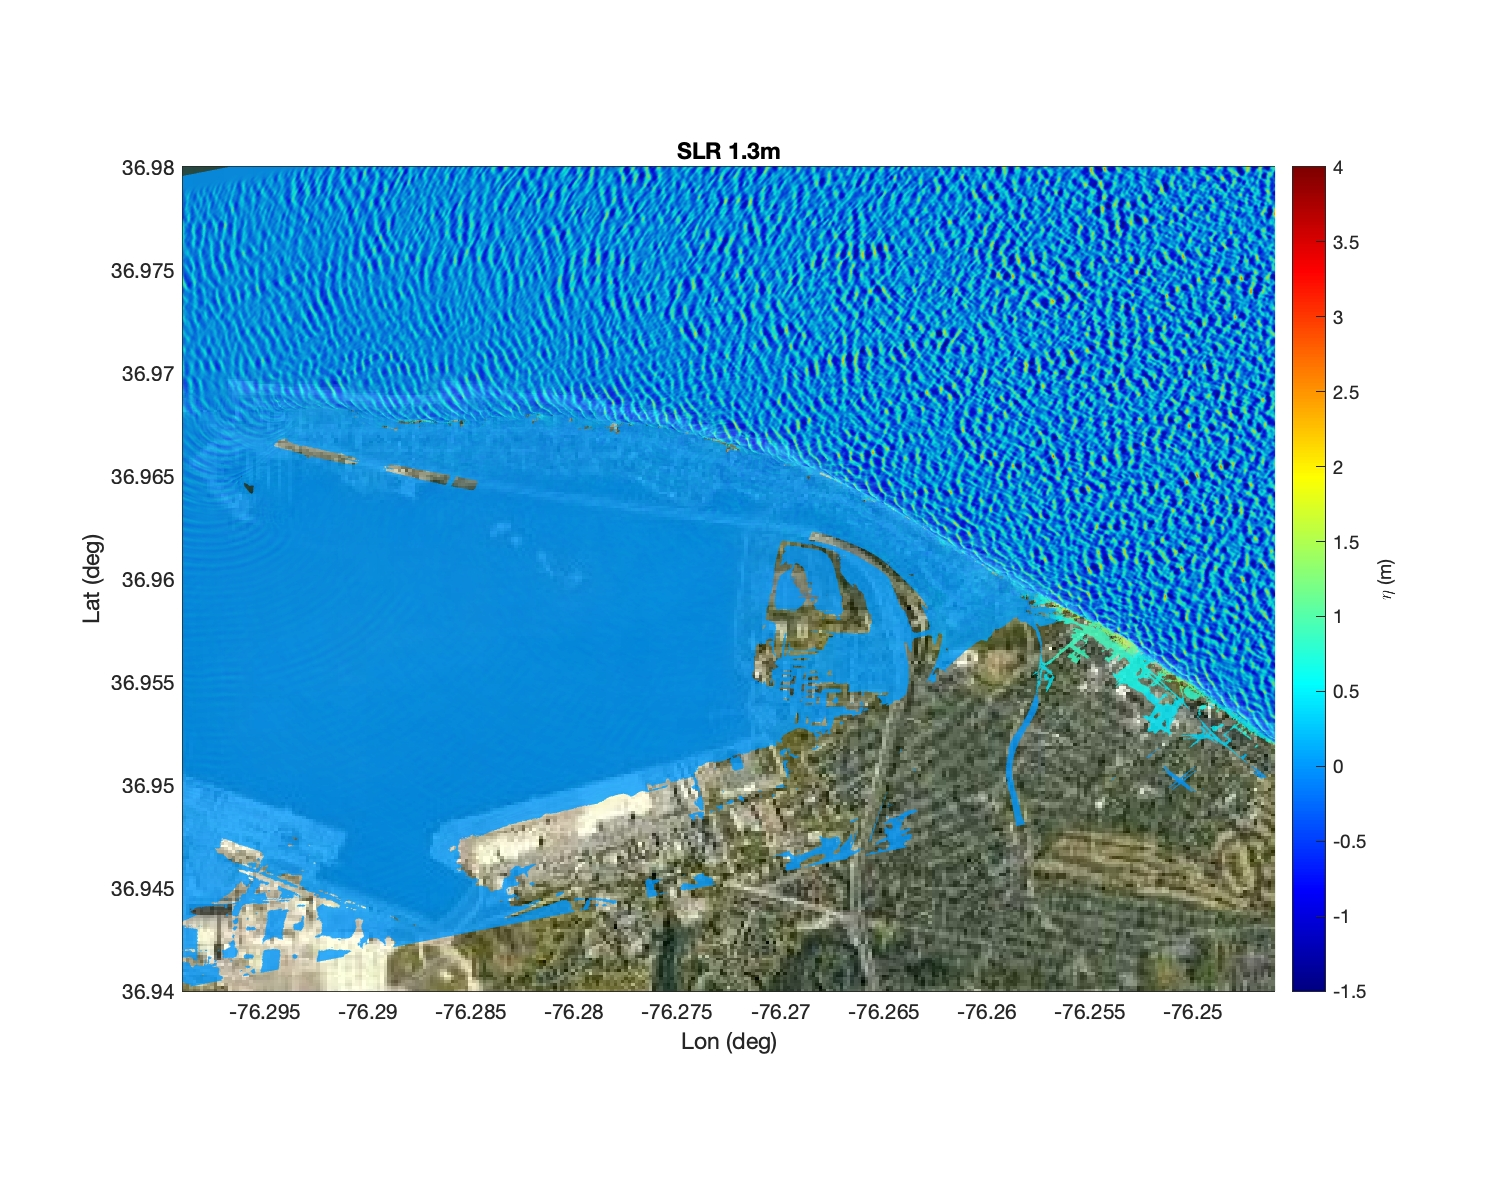
\includegraphics[width=\textwidth]{./figures/funwave_SLR _eta.jpg}
\caption{xxx }
\label{boundary}
\centering
\end{figure}

\begin{figure}
\centering
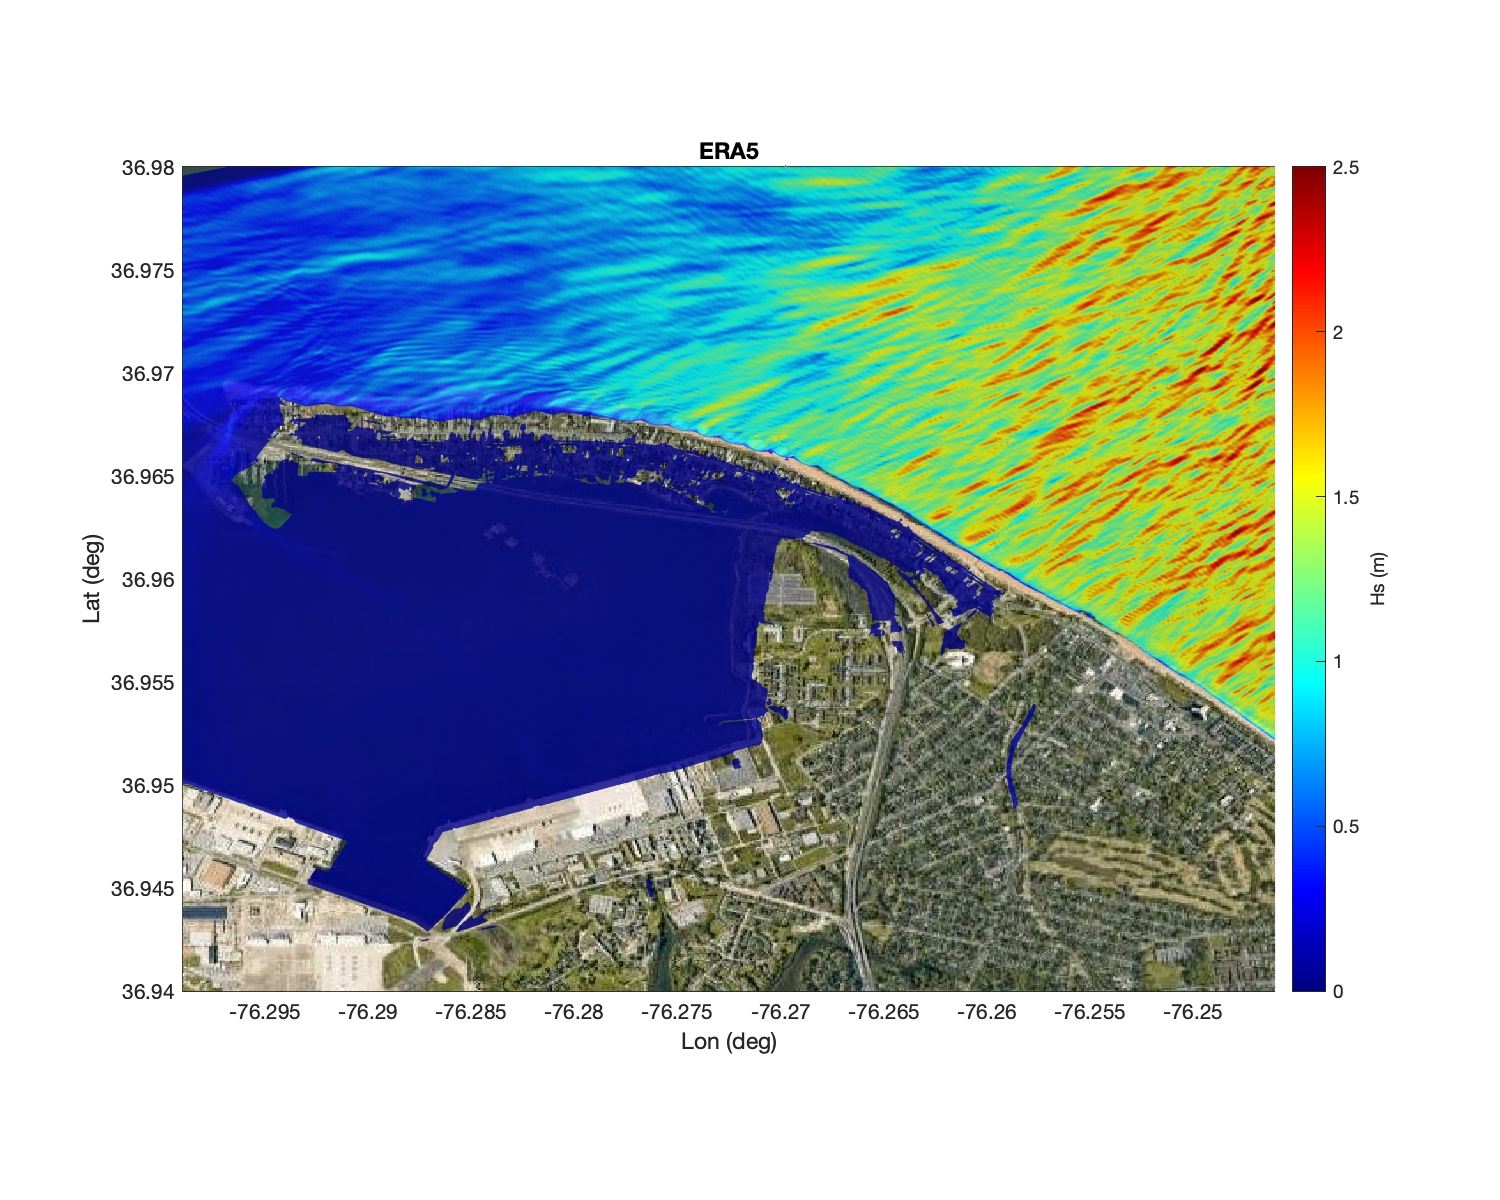
\includegraphics[width=\textwidth]{./figures/funwave_ERA5_hs.jpg}
\caption{xxx }
\label{boundary}
\centering
\end{figure}

\begin{figure}
\centering
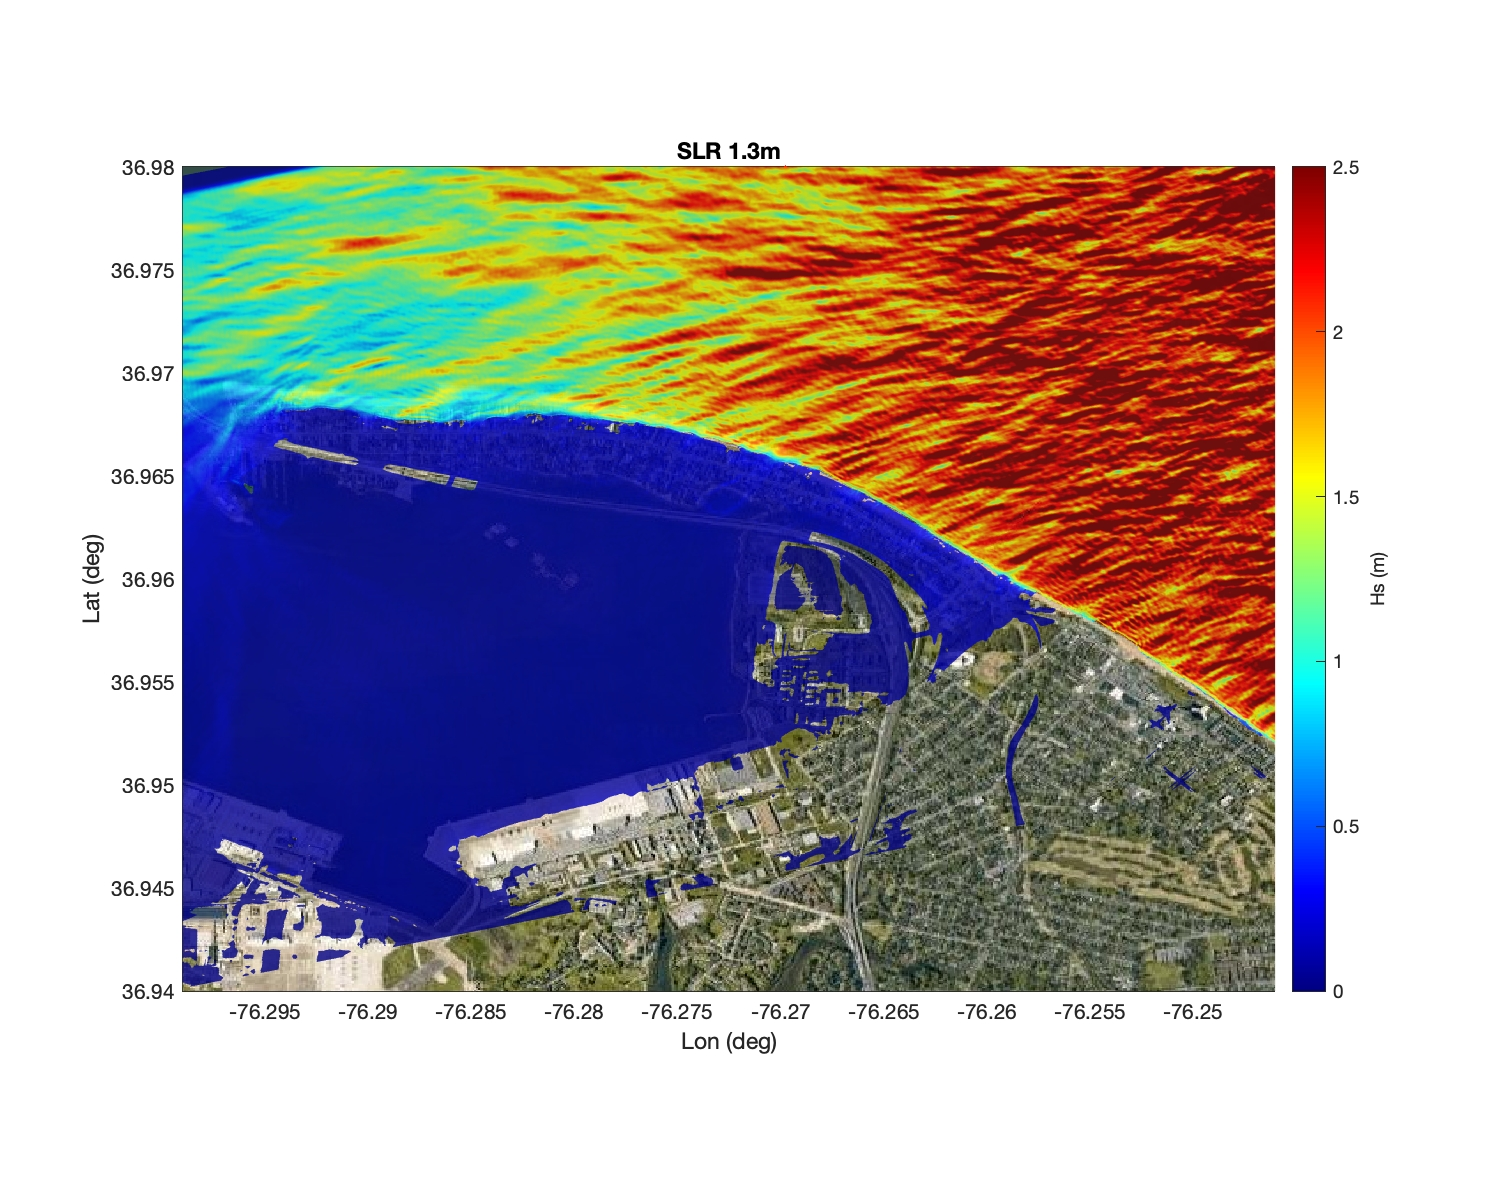
\includegraphics[width=\textwidth]{./figures/funwave_SLR_hs.jpg}
\caption{xxx }
\label{boundary}
\centering
\end{figure}

\begin{figure}
\centering
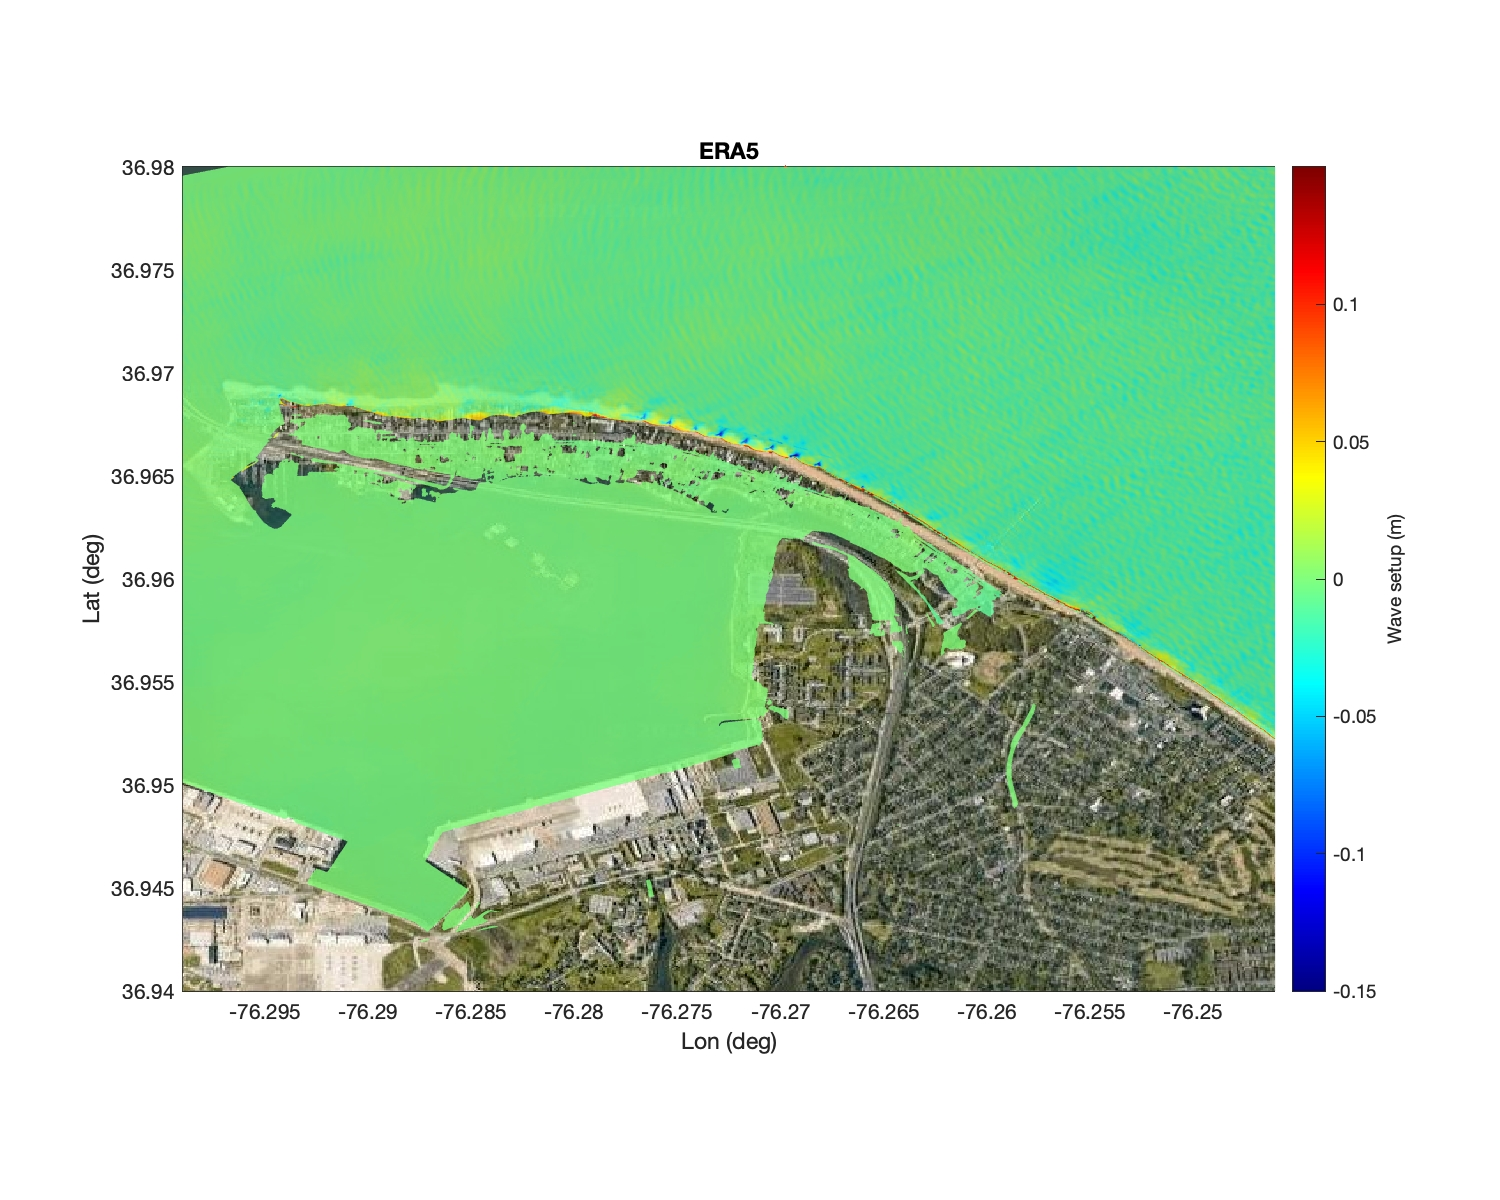
\includegraphics[width=\textwidth]{./figures/funwave_ERA5_setup.jpg}
\caption{xxx }
\label{boundary}
\centering
\end{figure}

\begin{figure}
\centering
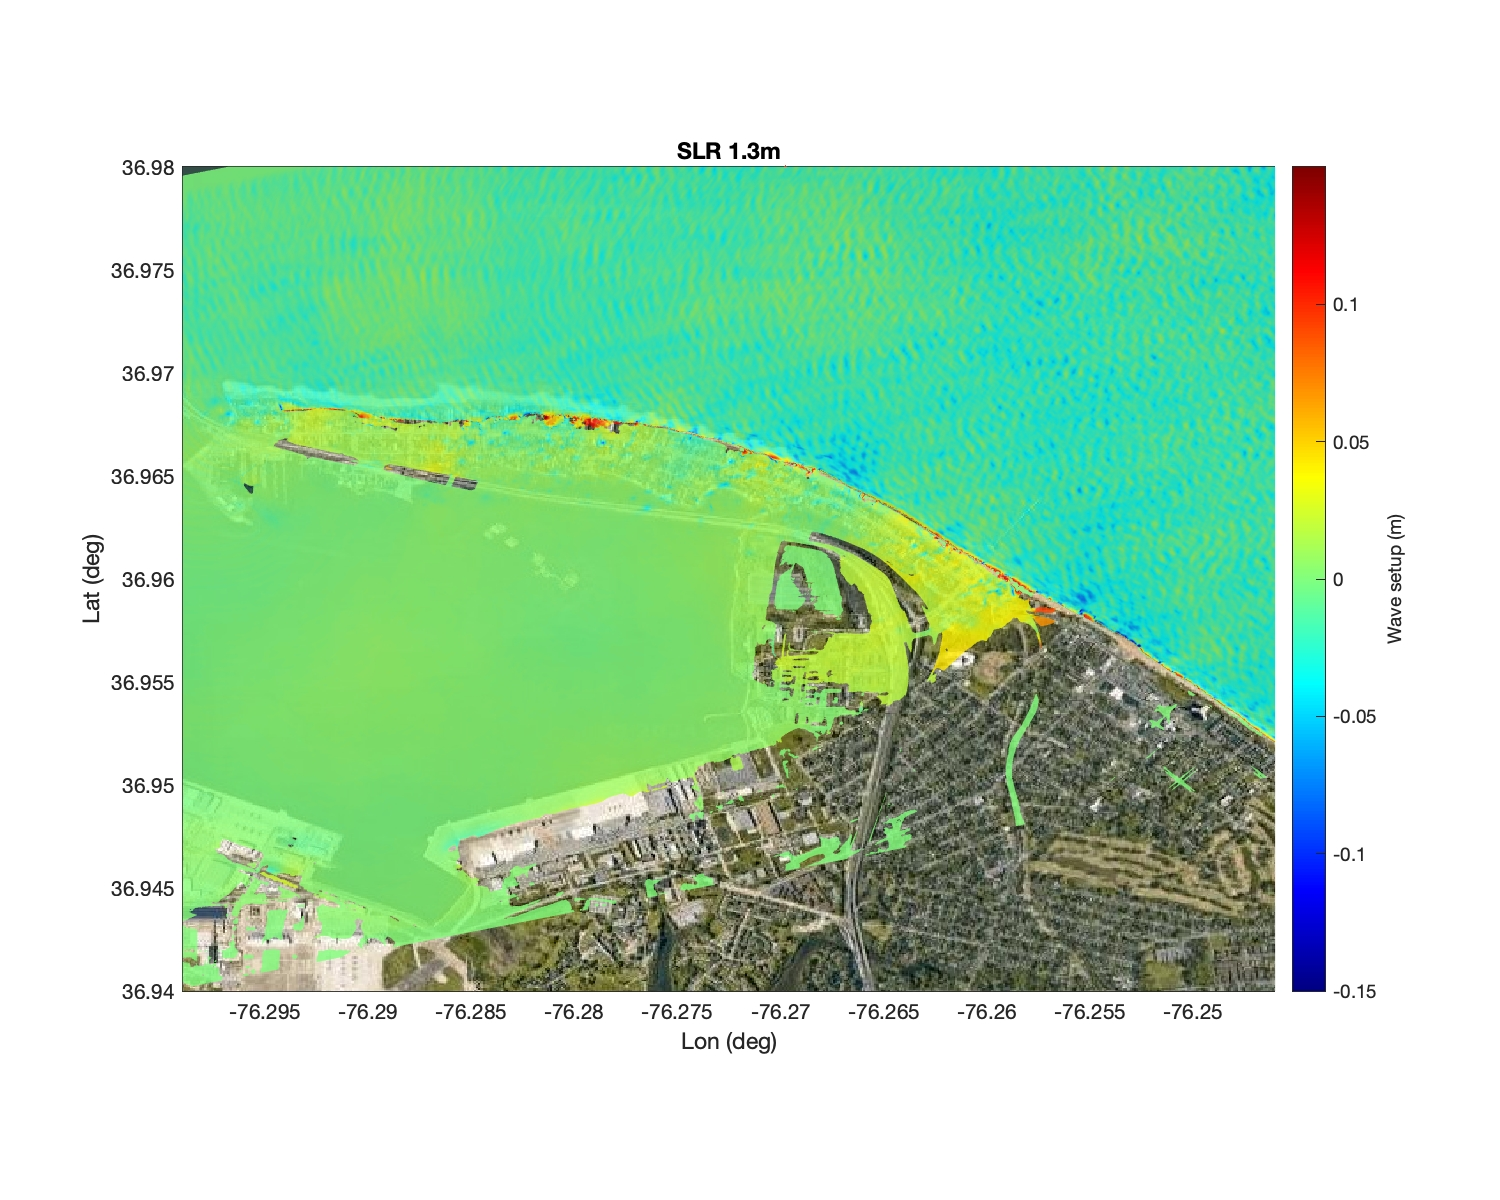
\includegraphics[width=\textwidth]{./figures/funwave_SLR_setup.jpg}
\caption{xxx }
\label{boundary}
\centering
\end{figure}

\begin{figure}
\centering
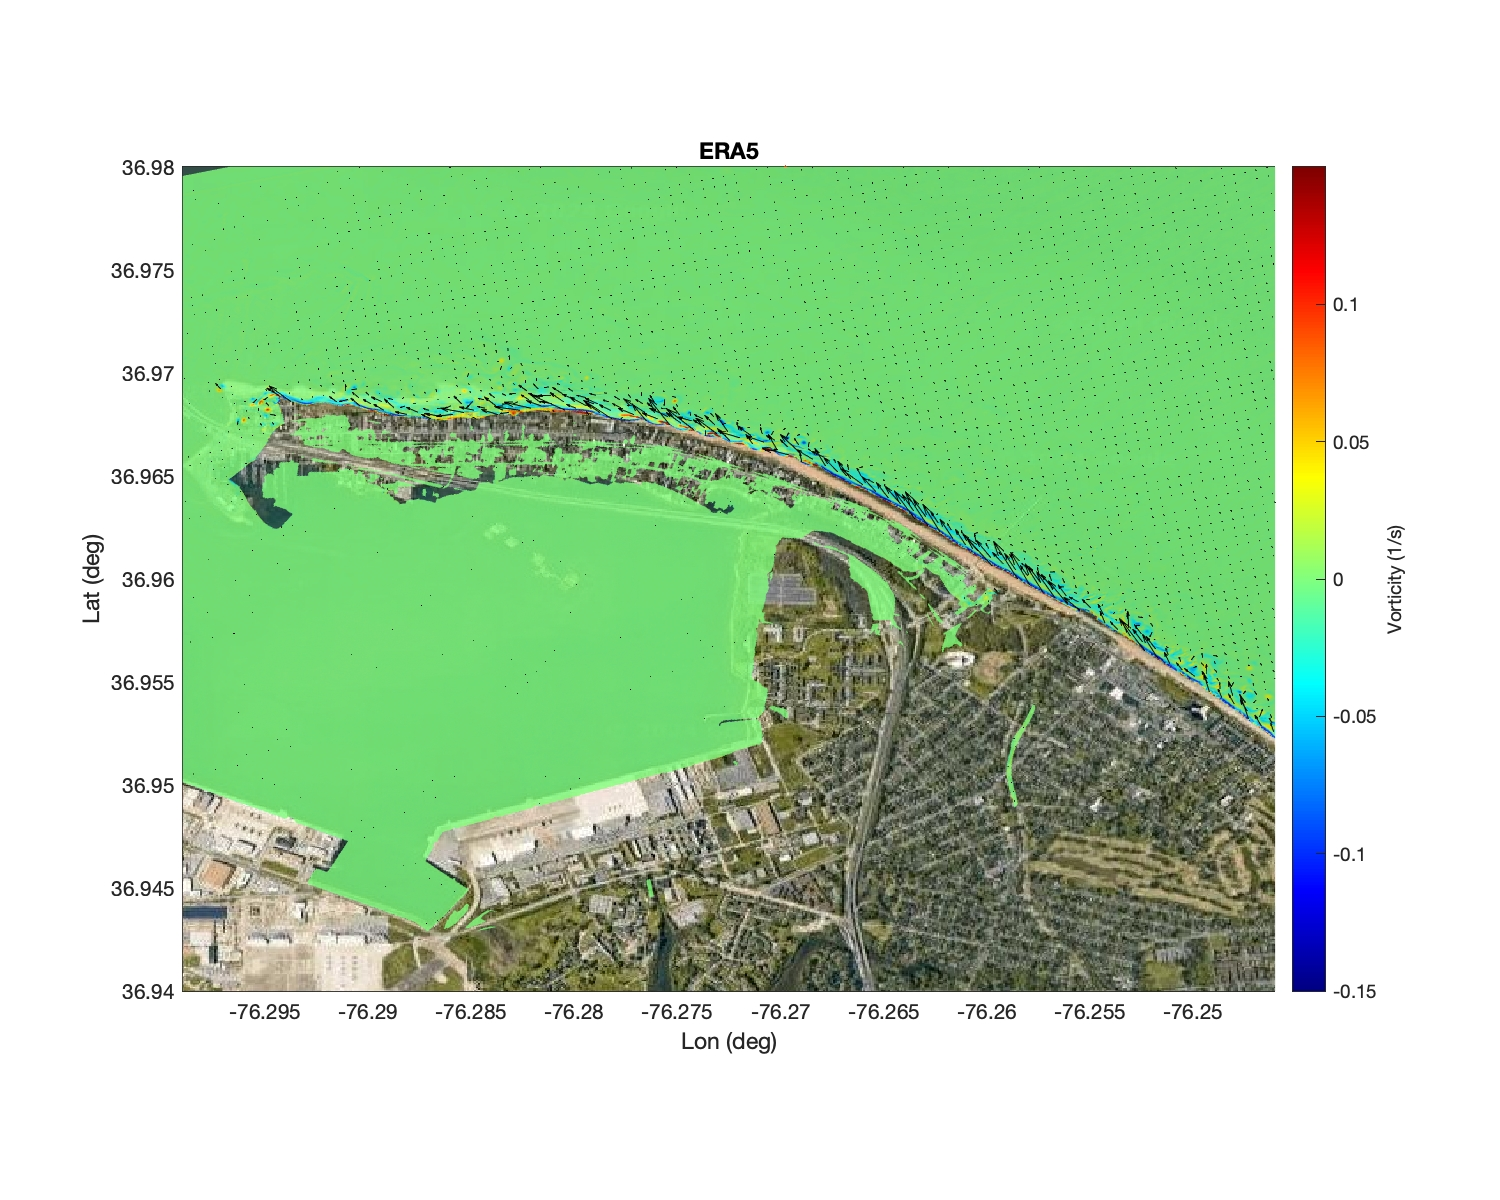
\includegraphics[width=\textwidth]{./figures/funwave_ERA5_vort.jpg}
\caption{xxx }
\label{boundary}
\centering
\end{figure}

\begin{figure}
\centering
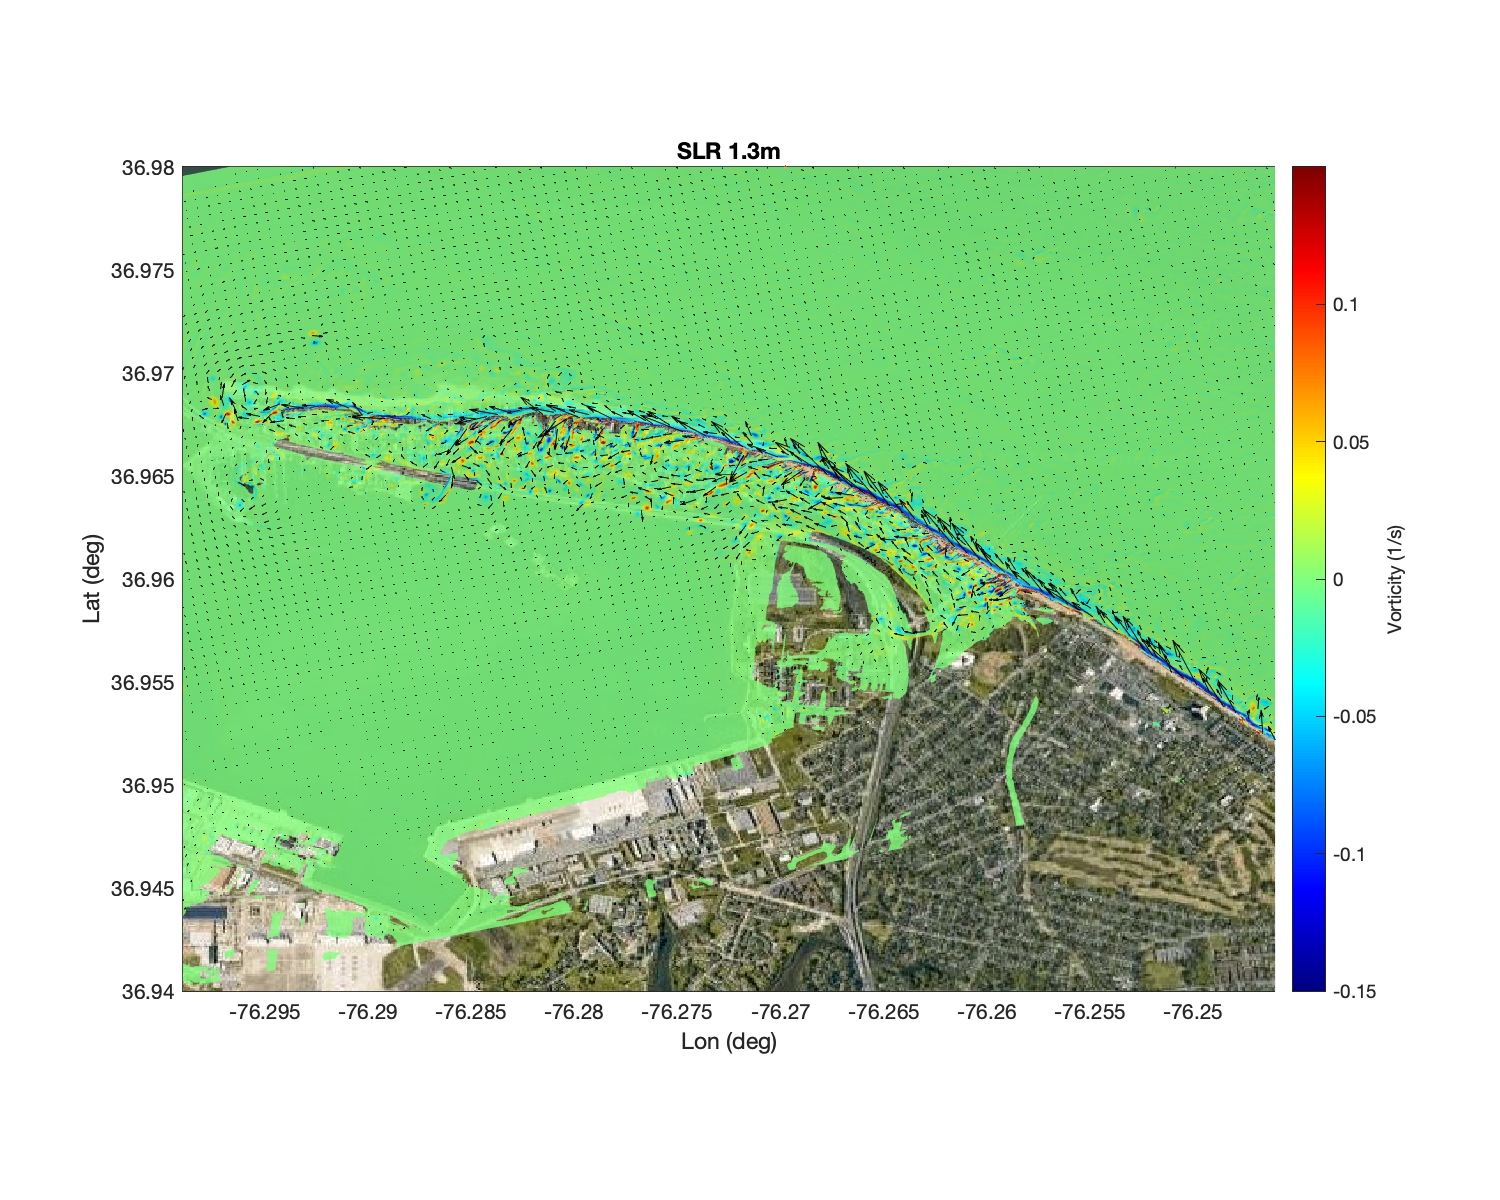
\includegraphics[width=\textwidth]{./figures/funwave_SLR_vort.jpg}
\caption{xxx }
\label{boundary}
\centering
\end{figure}

\begin{figure}
\centering
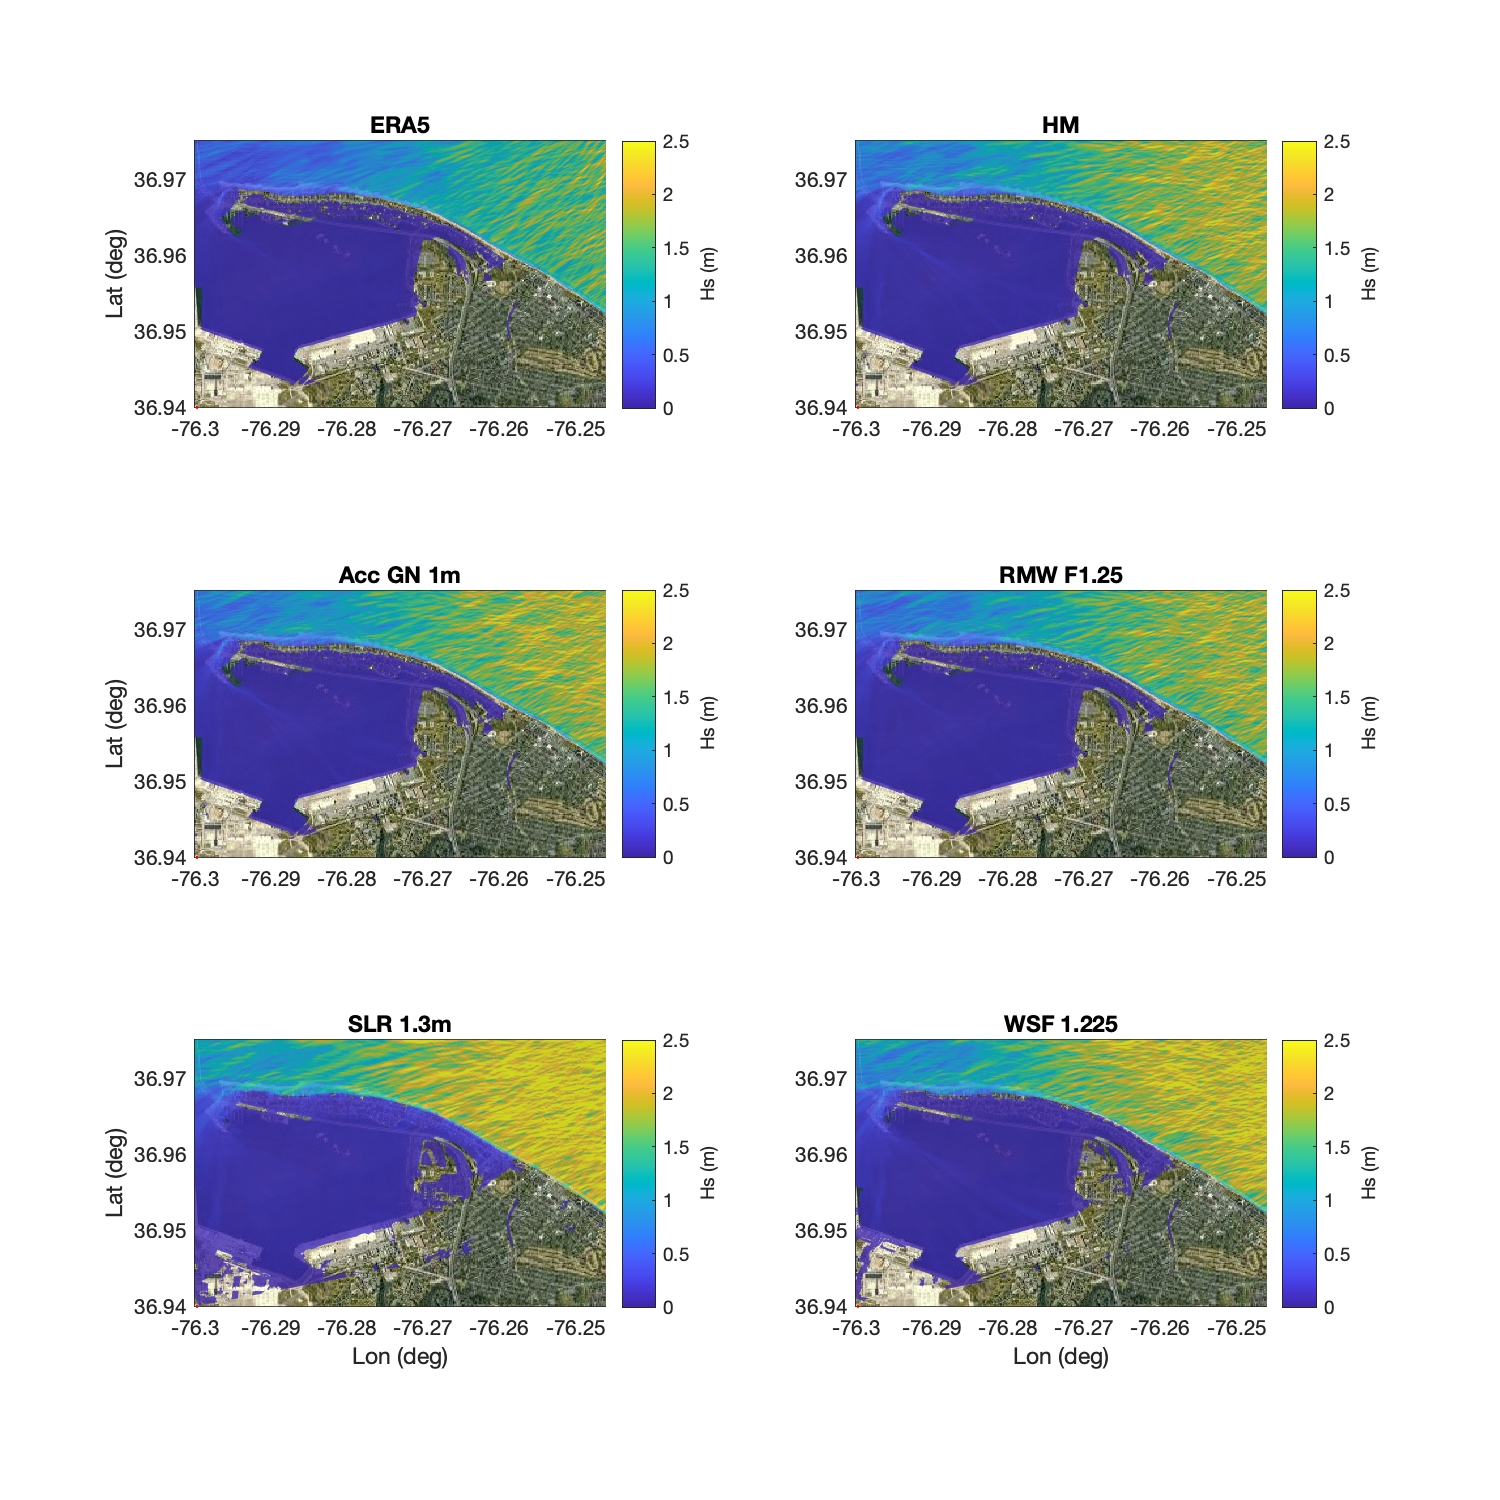
\includegraphics[width=\textwidth]{./figures/funwave_hs_6_cases.jpg}
\caption{xxx }
\label{boundary}
\centering
\end{figure}

\begin{figure}
\centering
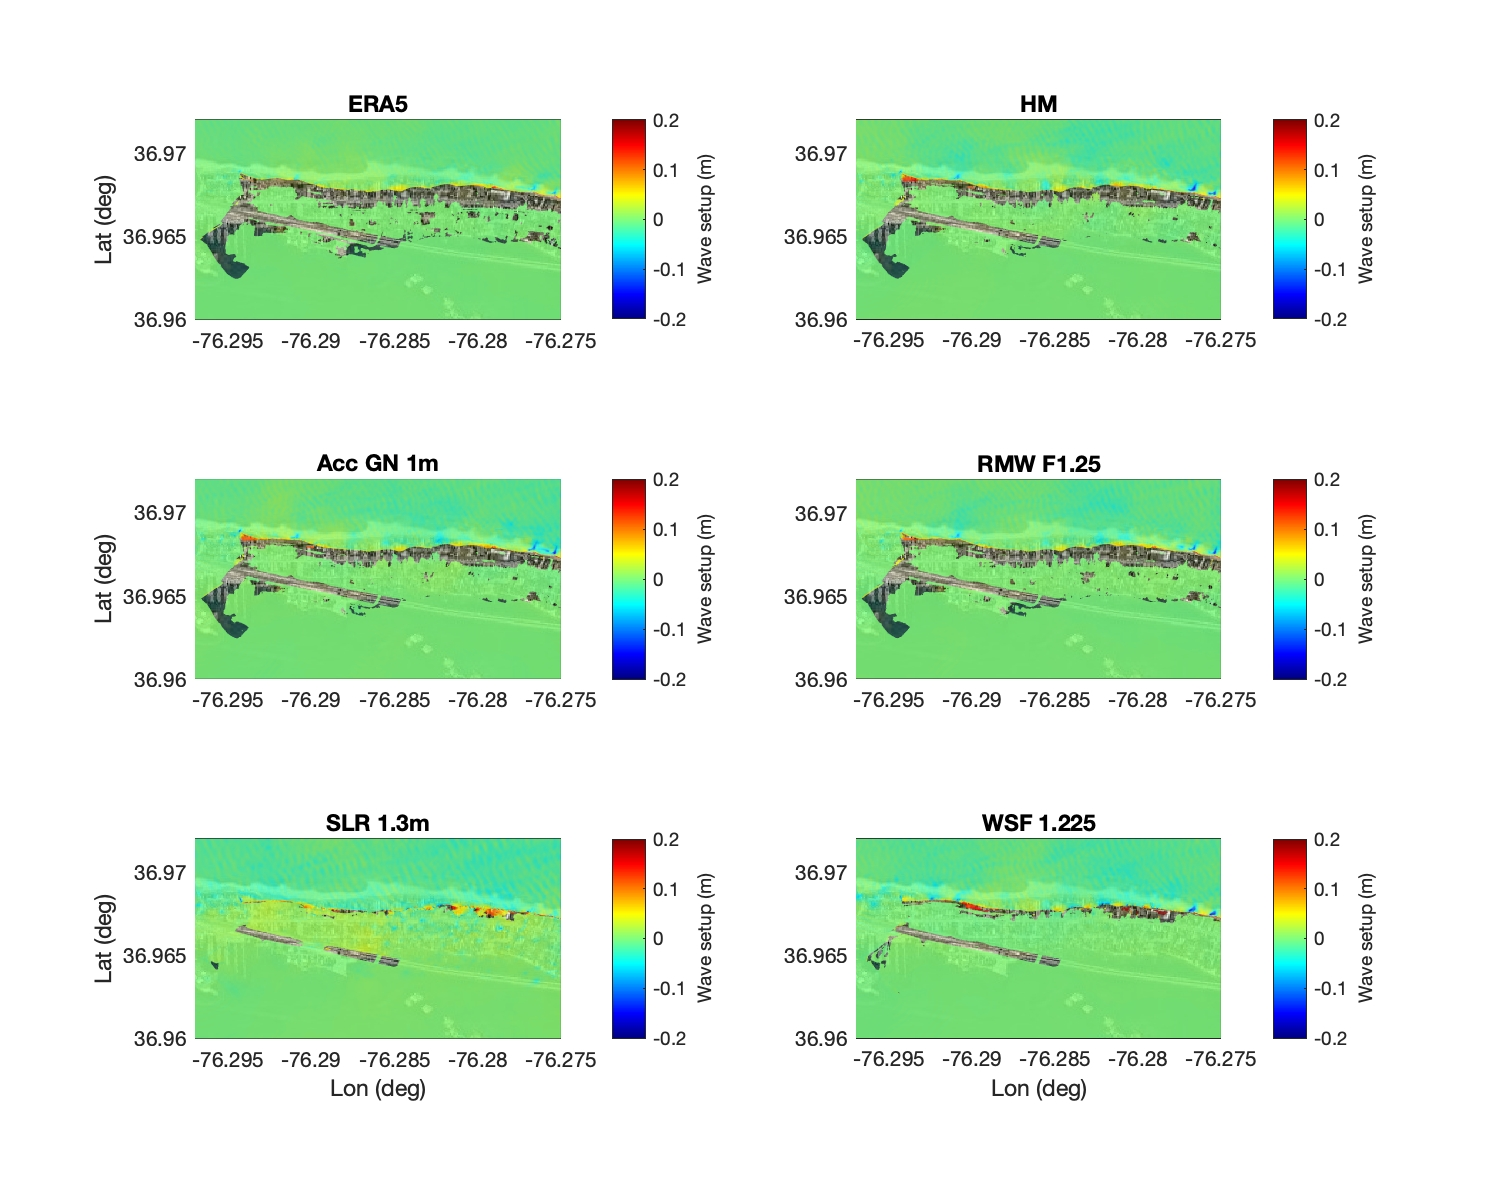
\includegraphics[width=\textwidth]{./figures/funwave_setup_6_cases.jpg}
\caption{xxx }
\label{boundary}
\centering
\end{figure}

\begin{figure}
\centering
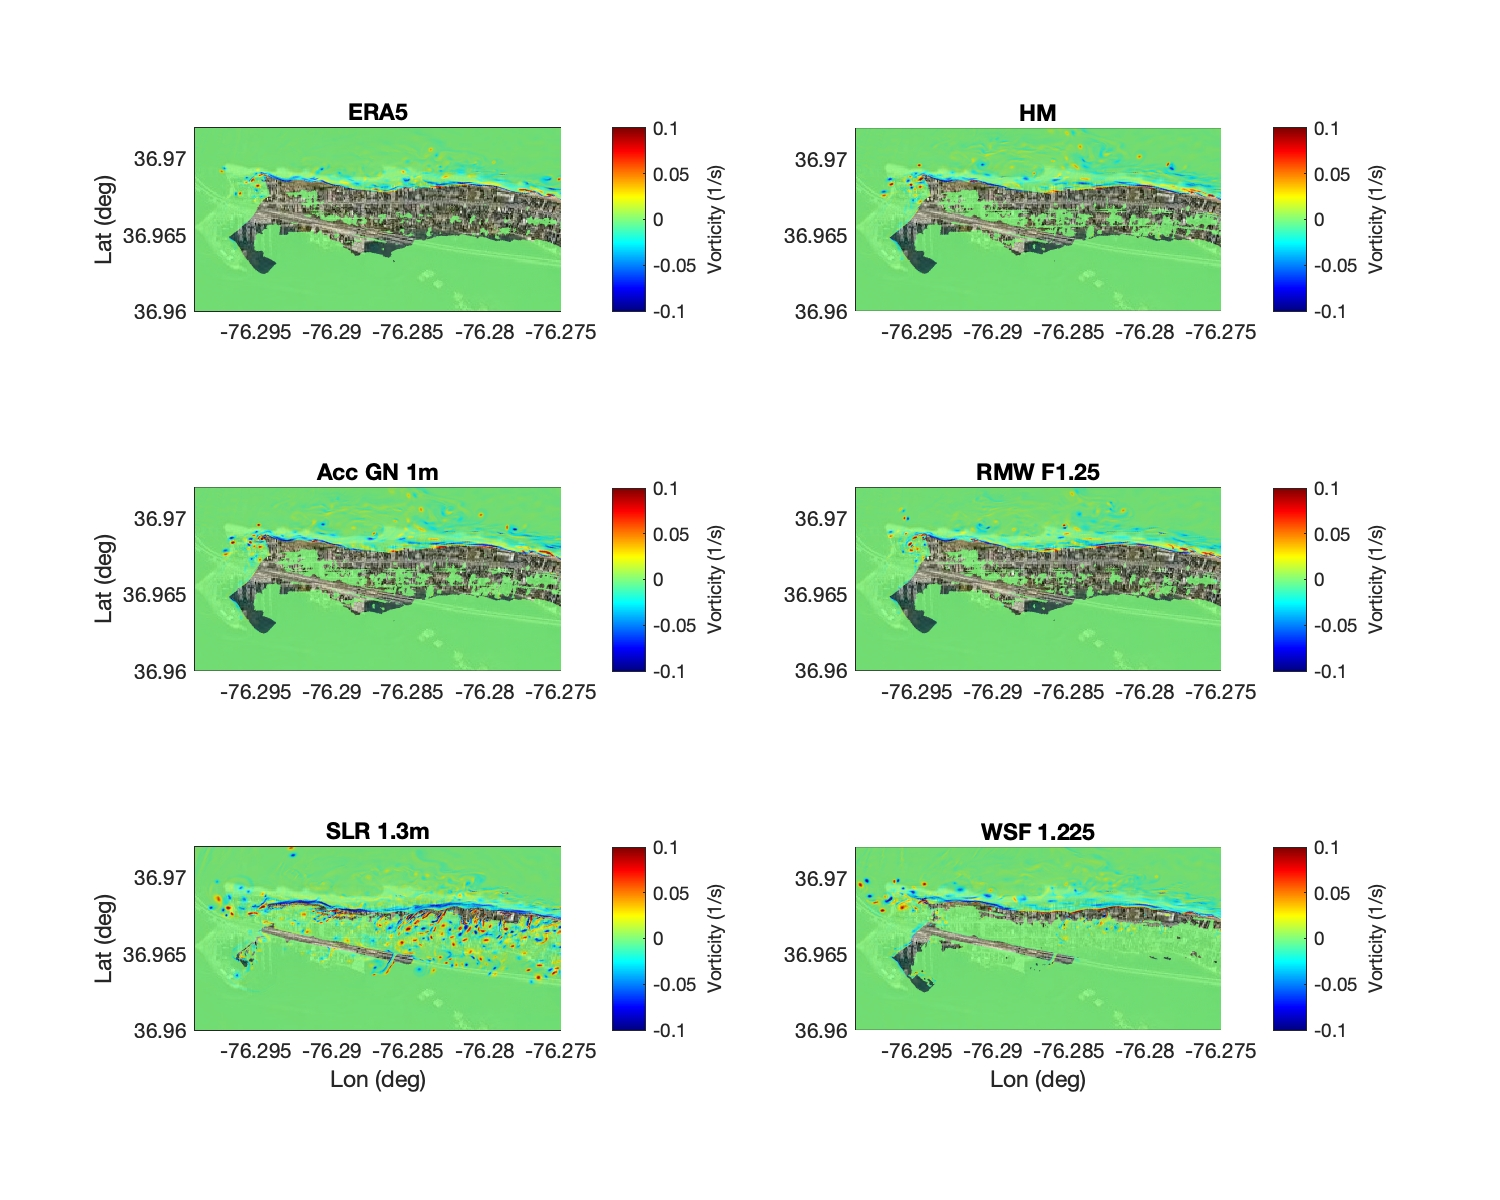
\includegraphics[width=\textwidth]{./figures/funwave_vort_6_cases.jpg}
\caption{xxx }
\label{boundary}
\centering
\end{figure}

\bibliographystyle{elsarticle-harv}

\biboptions{authoryear}
%\bibliographystyle{elsarticle-num}
\bibliography{bbh}
\end{document}